% =====================================================================
%  FAMIPET — PROJECT BLACK BOOK
%  Compiled with: latexmk -xelatex -interaction=nonstopmode main.tex
% =====================================================================
\documentclass[12pt,a4paper,twoside,openright]{book}

% ---------------------------------------------------------------
% Layout: binding-aware two-sided margins
% ---------------------------------------------------------------
\usepackage[a4paper,inner=1.30in,outer=0.90in,top=0.90in,bottom=0.90in,footskip=0.5in]{geometry}

% ---------------------------------------------------------------
% Fonts: 12 pt Times New Roman (body), DejaVu Sans Mono (code)
% ---------------------------------------------------------------
\usepackage{fontspec}
\setmainfont{Times New Roman}
\setmonofont{DejaVu Sans Mono}

% ---------------------------------------------------------------
% Supporting packages (strict black-and-white only)
% ---------------------------------------------------------------
\usepackage{graphicx}
\usepackage{booktabs}
\usepackage{longtable}
\usepackage{array}
\usepackage{tabularx}
\usepackage{ragged2e}
\usepackage{enumitem}
\setlist{topsep=2pt,itemsep=2pt,parsep=0pt,leftmargin=1.5em}
\usepackage{seqsplit}
\newcommand{\path}[1]{\texttt{\seqsplit{#1}}}
\usepackage{caption}
\captionsetup{font=small,labelfont=bf,labelsep=period,skip=6pt}
\usepackage{amsmath}
\usepackage{microtype}

% ---------------------------------------------------------------
% References: bibtex-driven. The stock \bibliography inputs the .bbl
% under the \jobname and emits its own "Bibliography" \chapter heading;
% \famibid writes the bibstyle/bibdata hints to the aux so bibtex runs,
% then calls the stock \bibliography while locally swallowing any
% \chapter (the REFERENCES opener already opened the heading) so the
% .bbl's list appears directly beneath it without a second heading.
% ---------------------------------------------------------------
\makeatletter
\def\famigobblechapter{\@ifstar{\@gobble}{\@gobble}}
\newcommand{\famibid}[1]{%
  \immediate\write\@auxout{\string\bibstyle{ieeetr}}%
  \begingroup
  \let\chapter\famigobblechapter
  \let\famigobblechapter\@undefined
  \bibliography{#1}%
  \endgroup
}
\makeatother

% ---------------------------------------------------------------
% Headers / footers: page number bottom, odd-right, even-left
% ---------------------------------------------------------------
\usepackage{fancyhdr}
\pagestyle{fancy}
\fancyhf{}
\fancyfoot[LE,RO]{\thepage}
\renewcommand{\headrulewidth}{0pt}

% ---------------------------------------------------------------
% Chapter-opening pages
%  - every chapter starts on a right-hand (odd) page
%  - the opening page contains ONLY chapter number, title and a
%    short description, and carries no page number
%  - genuine blank forcing pages (no number, no decoration)
% ---------------------------------------------------------------
\newcommand{\cleartorecto}{\clearpage{\pagestyle{empty}\cleardoublepage}}

\newcommand{\famichapter}[3]{%
  \cleartorecto
  \thispagestyle{empty}%
  \global\stepcounter{chapter}%
  \addcontentsline{toc}{chapter}{\protect\numberline{\thechapter}#1}%
  \setcounter{section}{0}%
  \setcounter{figure}{0}%
  \setcounter{table}{0}%
  \setcounter{footnote}{0}%
  \begin{center}
    \vspace*{\fill}
    {\fontsize{14}{17}\selectfont\bfseries CHAPTER \thechapter\par}
    \vspace{10pt}
    {\fontsize{20}{24}\selectfont\bfseries\MakeUppercase{#1}\par}
    \vspace{18pt}
    {\normalsize #2\par}
    \vspace*{\fill}
  \end{center}
  \clearpage
  \label{#3}%
}

\newcommand{\famichapterstar}[3]{%
  \cleartorecto
  \thispagestyle{empty}%
  \addcontentsline{toc}{chapter}{#1}%
  \begin{center}
    \vspace*{\fill}
    {\fontsize{20}{24}\selectfont\bfseries\MakeUppercase{#1}\par}
    \vspace{18pt}
    {\normalsize #2\par}
    \vspace*{\fill}
  \end{center}
  \clearpage
  \label{#3}%
}

% ---------------------------------------------------------------
% Hyperlinks: never colored (black book rule)
% ---------------------------------------------------------------
\usepackage[hidelinks]{hyperref}

% ---------------------------------------------------------------
% Front matter page numbering (roman)
% ---------------------------------------------------------------
\newcommand{\frontpagestyle}{\clearpage{\pagestyle{empty}\cleardoublepage}\pagenumbering{roman}}

\begin{document}

% ---------------- TOC / LOF / LOT ----------------
\frontpagestyle
\renewcommand{\contentsname}{CONTENTS}
\tableofcontents
\clearpage
\renewcommand{\listfigurename}{LIST OF FIGURES}
\listoffigures
\clearpage
\renewcommand{\listtablename}{LIST OF TABLES}
\listoftables
\clearpage

% ---------------- GLOSSARY (front matter) ----------------
\renewcommand{\sectionmark}[1]{}
\famichapterstar{Glossary of Terms and Abbreviations}{Definitions of the
technical terms and abbreviations used throughout this black book.}{ch:glossary}
\section*{Terms}

\begin{center}
\begin{longtable}{@{}p{3.4cm}p{11.2cm}@{}}
\toprule
\textbf{Term} & \textbf{Definition} \\
\midrule
API & Application Programming Interface; in FamiPet, the HTTP/REST surface of
the backend under \texttt{/api/*}. \\
Bcrypt & A password-hashing function; FamiPet uses cost factor 12 and verifies
login passwords against the stored hash. \\
Bearer token & The JWT sent in the \texttt{Authorization: Bearer} header on
protected requests. \\
Controller & Backend module implementing validation, ownership checks, and
business effects for one subsystem. \\
CORS & Cross-Origin Resource Sharing; the backend origin guard that allows only
the configured client, localhost, and private LAN origins. \\
CRUD & Create, Read, Update, Delete; the basic data operations exposed by the
API. \\
Digital pet identity & The unique \texttt{petUid} plus the QR code generated for
each pet. \\
Document & A record in MongoDB, represented in code by a Mongoose model. \\
E2E & End-to-end; testing through the real browser and HTTP surface. \\
JWT & JSON Web Token (RFC 7519); the signed token that authenticates requests. \\
Mongoose & The object-document mapper used by the backend to define schemas,
indexes, and queries on MongoDB. \\
Multer & Middleware that parses multipart image uploads, restricted to JPEG, PNG,
and WebP, up to 5\,MB. \\
Nodemailer & The e-mail library used to send verification and password-reset
messages over SMTP. \\
ObjectId & MongoDB's 24-character hexadecimal document identifier. \\
ODM & Object-Document Mapper; conversion layer between MongoDB documents and
JavaScript objects. \\
Owner-scoped query & A database query that binds results to the authenticated
user (\texttt{user: req.user.\_id}). \\
petUid & The unique digital pet identifier embedded in the QR code. \\
Populate & Mongoose operation that replaces a referenced \texttt{ObjectId} with
the referenced document. \\
protect / adminOnly & The authentication and role middleware pair. \\
QR code & Quick Response code; encodes the public pet identity payload as a PNG
data URL. \\
REST & Representational State Transfer; the API style used by the platform. \\
Scheduler & A mechanism that would run periodic jobs; declared in dependencies
but not implemented. \\
SHA-256 & The hash used to store e-mail verification and password-reset tokens,
so plaintext tokens are never stored. \\
SMTP & Simple Mail Transfer Protocol, the transport used by Nodemailer. \\
\bottomrule
\end{longtable}
\addtocounter{table}{-1}
\end{center}

\section*{Abbreviations}

\begin{center}
\begin{longtable}{@{}p{3.4cm}p{11.2cm}@{}}
\toprule
\textbf{Abbreviation} & \textbf{Meaning} \\
\midrule
HTTP(S) & HyperText Transfer Protocol (Secure) \\
JSON & JavaScript Object Notation \\
HTML & HyperText Markup Language \\
CSS & Cascading Style Sheets \\
URI & Uniform Resource Identifier \\
DB & Database \\
LAN & Local Area Network \\
AI & Artificial Intelligence \\
QA & Quality Assurance \\
UI & User Interface \\
UX & User Experience \\
\bottomrule
\end{longtable}
\addtocounter{table}{-1}
\end{center}

% ---------------- MAIN MATTER ----------------
{\pagestyle{empty}\cleardoublepage}
\pagenumbering{arabic}
\setcounter{page}{1}

\famichapter{Introduction}{This chapter introduces FamiPet, a pet-care and adoption
platform. It describes the purpose of the project, the scope of this black book, the
overall system context, and the document structure.}{ch:intro}

\section{Project Overview}

FamiPet is a full-stack web application that supports pet owners, prospective
adopters, and platform administrators. The application lets registered users
maintain profiles for their pets, generate a digital pet identity with a QR code,
record health and vaccination information, book veterinary appointments, set
medication and care reminders, participate in a community, report lost or found
animals, and apply to adopt pets listed on the platform. An administrator can
moderate content, manage users, and process adoption requests.

The system is built as a client--server application. The backend is a Node.js~\cite{nodejs}
application written with Express~\cite{express} that exposes a REST API and persists all data in
MongoDB through the Mongoose object-document mapper. The frontend is a React and
TypeScript web application built with Vite and Tailwind CSS; it communicates with
the backend over HTTP, and the backend remains the source of truth for all data
and business rules.

\section{Purpose of this Document}

This black book is a formal academic record of the FamiPet project. It documents,
from the actual implementation:

\begin{itemize}
    \item the problem the project addresses and its objectives;
    \item the functional and non-functional requirements and the system scope;
    \item the analysis and design of the system;
    \item the system architecture and deployment;
    \item the data model stored in MongoDB;
    \item the authentication, authorization, and security mechanism;
    \item the core features and their workflows;
    \item the implementation structure and technology stack;
    \item the testing performed and its evidence;
    \item the development process followed;
    \item conclusions and future work.
\end{itemize}

Every statement about behaviour, data, security, and testing in this document is
derived from the verified implementation in the repository. Planned work, such as
the remaining roadmap phases described in Chapter~\ref{ch:conclusion}, is
explicitly identified as planned rather than as delivered functionality.

\section{System Context}

Figure~\ref{fig:system-context} shows the context of the system. The backend API
is the central component: it receives HTTP requests from the frontend, applies
authentication and ownership rules, and persists and retrieves data in MongoDB.
It also integrates with external services for e-mail delivery, AI-powered pet
care assistance, and image processing.

\begin{figure}[htbp]
    \centering
    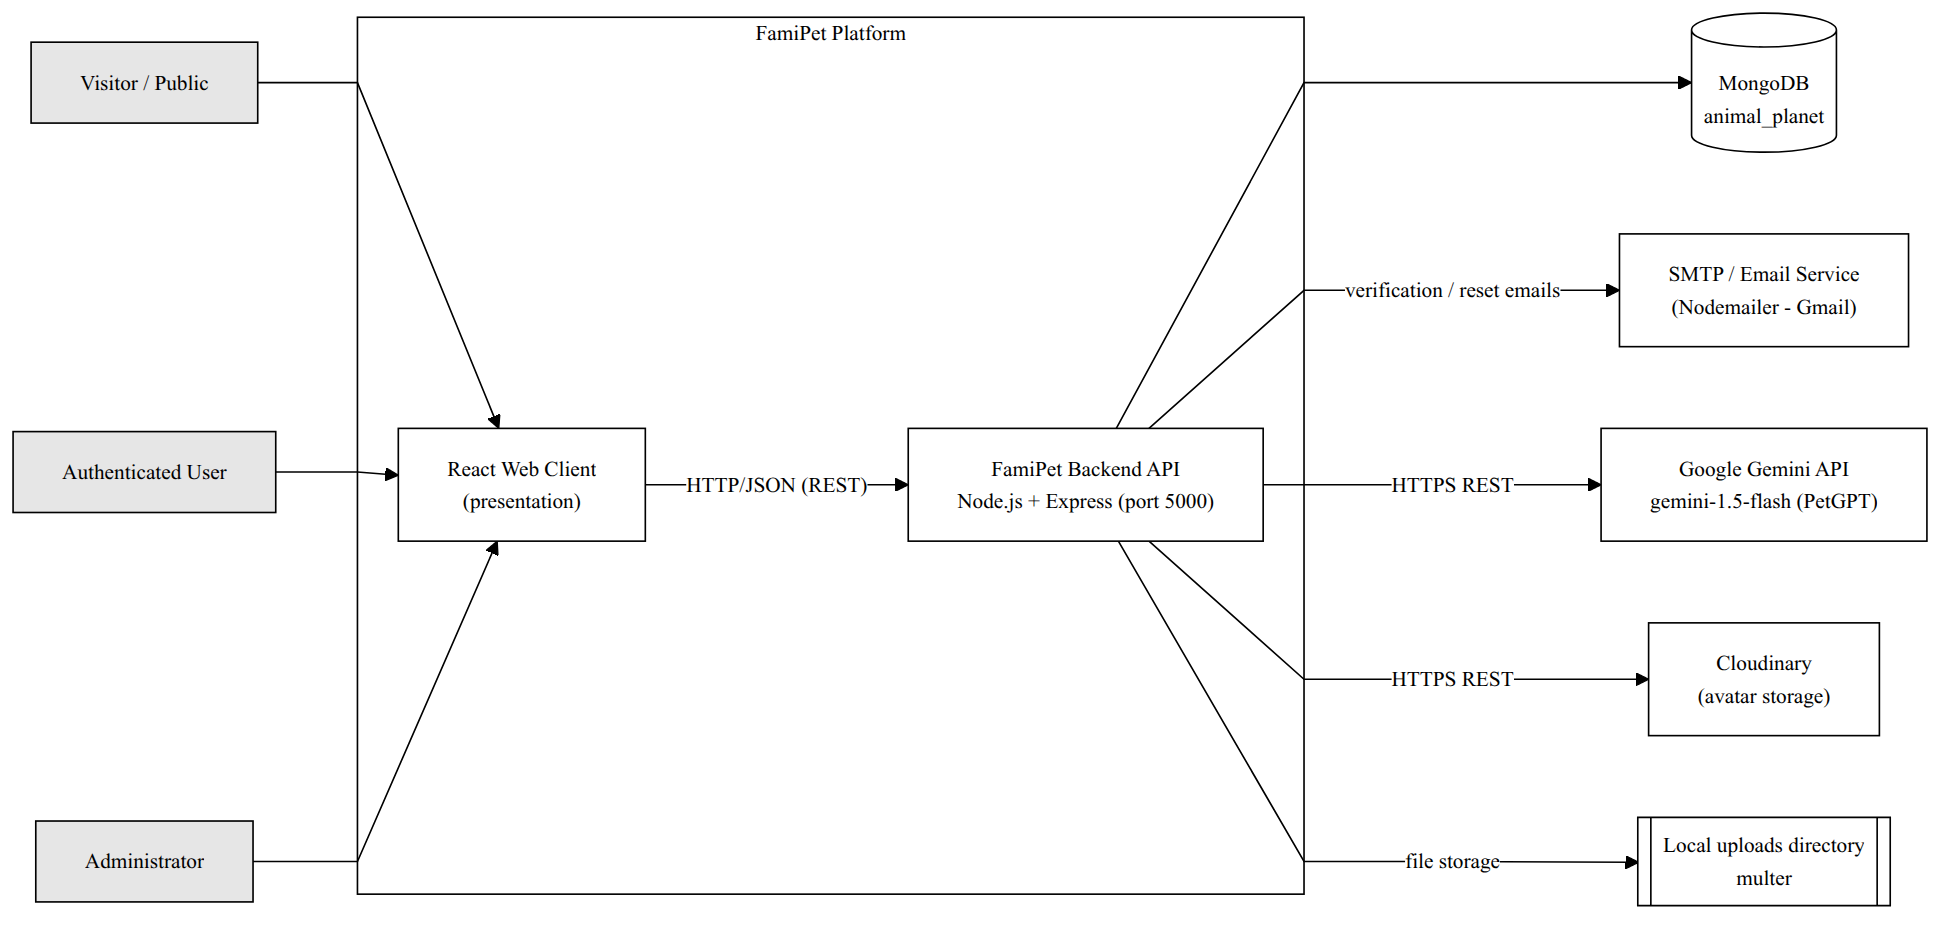
\includegraphics[width=\textwidth]{figures/01-system-context.png}
    \caption{FamiPet system context diagram.}
    \label{fig:system-context}
\end{figure}

The context diagram shows four external parties. The \emph{React web client}
interacts with the platform through the public HTTP API; the \emph{MongoDB}
database stores
all records; the \emph{e-mail service} (Nodemailer over SMTP) delivers account
verification and password-reset messages; and the \emph{Google Gemini} AI service
provides the conversational pet-care assistant. Uploaded images are stored on
Cloudinary when credentials are configured and served locally from the
\texttt{uploads} directory otherwise.

\section{Document Structure}

The black book is organised as follows. Chapter~2 defines the problem and
objectives. Chapter~3 presents the requirement specification and scope, including
functional and non-functional requirements, user roles, and use cases.
Chapter~4 analyses the system and the technology stack. Chapter~5 describes the
architecture and design. Chapter~6 documents the MongoDB data model. Chapter~7
describes authentication, authorization, and security. Chapter~8 explains the
core features and their workflows. Chapter~9 describes the implementation
structure. Chapter~10 records the testing and validation evidence. Chapter~11
documents the development process. Chapter~12 presents the conclusion and future
scope. The list of terms and abbreviations appears before the main matter;
references and two appendices conclude the black book.
\famichapter{Problem and Objectives}{This chapter defines the problem that FamiPet
addresses, the objectives of the project, and the deliverables that define a
successful implementation.}{ch:problem}

\section{Problem Statement}

Pet ownership involves several practical responsibilities that are today spread
across separate tools and sources: remembering vaccination schedules, tracking
medical history, keeping appointments with veterinarians, organising daily care
like feeding and medicine, proving a pet's identity when it is lost, and managing
the process of adopting an animal responsibly. Owners keep this information
informally or in unrelated documents, so records are lost, reminders are missed,
and a pet's health history is unavailable at the moment it is needed. People
looking for a pet have similar difficulties: there is no single place to see
animals available for adoption and to apply for them, or to report and search
lost or found animals.

FamiPet addresses this by providing one integrated platform in which:

\begin{itemize}
    \item a user registers, verifies the account, and manages a personal profile;
    \item a user records pets, generating a unique digital pet identity and a QR
    code that encodes public pet information;
    \item health records and vaccinations are kept per pet, with ownership
    enforced by the backend;
    \item veterinary appointments can be booked against a veterinarian's
    availability, with automatic notifications and reminders;
    \item reminders for feeding, medicine, grooming, and care can be created and
    completed;
    \item users can post to a community, like and comment on posts, and report
    lost or found animals;
    \item users can apply to adopt pets, and administrators can approve or reject
    those applications, automatically changing the pet's status; and
    \item an AI assistant answers pet-care questions and gives advice based on
    the user's actual pet records.
\end{itemize}

The problem is therefore the need for an authenticated, backend-driven pet-care
system in which all user data is owned by the correct user, is persisted in a
real database, and is protected by server-side access control.

\section{Objectives}

The objectives of the FamiPet project are:

\begin{enumerate}
    \item To build a full-stack web application for pet care and adoption with an
    authenticating backend and a database-backed data store.
    \item To provide a secure authentication mechanism based on e-mail
    verification, password hashing, and signed bearer tokens.
    \item To enforce ownership and role-based authorization on the backend so
    that users can only access their own resources and only administrators can
    perform administrative actions.
    \item To implement a digital pet identity with a unique pet identifier and a
    QR code that can be read to obtain public pet information.
    \item To implement pet health management, including health records and
    vaccinations, tied to the authenticated owner's pets.
    \item To implement appointment booking with veterinarian slot conflict
    detection and automatic notification and reminder generation.
    \item To implement a reminder system with per-owner, per-pet reminders that
    persist and can be completed.
    \item To implement adoption management with pending, approved, and rejected
    states and automated pet status transitions and notifications.
    \item To implement community and lost-and-found features with moderation by
    administrators.
    \item To integrate an AI pet-care assistant that uses the owner's real pet
    data and falls back to safe, generic guidance when the AI service is
    unavailable.
    \item To validate the system through real end-to-end tests, database
    persistence checks, and security boundary tests.
\end{enumerate}

\section{Deliverables and Success Criteria}

The project deliverables are:

\begin{itemize}
    \item the backend API (Express, MongoDB, Mongoose) at \texttt{backend/};
    \item the frontend application at \texttt{frontend/} and its in-progress
    React migration at \texttt{frontend-react/};
    \item project documentation, including this black book, the implementation
    roadmap (\texttt{ROADMAP.md}, \texttt{docs/migration.md}), and the
    maintenance rules in \texttt{AGENTS.md};
    \item a seeded database containing default breeds, an administrator account,
    and a demo user for evaluation.
\end{itemize}

A phase is considered successful when the functionality is implemented, connects
to the persisted database, passes the associated tests, and is committed and
pushed to the repository. Feature phases are tracked in a checklist: at the time
of writing, the vanilla frontend and backend are feature-complete, and React
migration phases 1--21 are complete while phases 22--29 remain planned
(Chapter~\ref{ch:process}).
\famichapter{Requirements and Scope}{This chapter specifies the functional and
non-functional requirements of FamiPet, the user roles and their permissions, the
scope of the system, and the use cases that the implementation supports.}{ch:req}

\section{Actors and Roles}

The system distinguishes three actors, defined by the actual implementation.

\begin{table}[htbp]
\centering
\begin{tabular}{@{}p{2.5cm}p{3.2cm}p{8.6cm}@{}}
\toprule
\textbf{Role} & \textbf{Stored as} & \textbf{Permissions enforced by the backend} \\
\midrule
Visitor & no account & Browse public content: pets, breeds, veterinarian
directory, community posts, and lost-and-found reports. Cannot create or modify
any resource. \\
\addlinespace
Registered user & \texttt{User.role = "user"} & All visitor permissions plus
account management, pet management with QR identity, health records,
vaccinations, appointments, reminders, favorites, community posts, lost-and-found
reports, adoption applications, notifications, and the AI assistant. \\
\addlinespace
Administrator & \texttt{User.role = "admin"} & All user permissions plus the
admin panel: dashboard statistics, user management and blocking, pet moderation,
adoption approval/rejection, community and lost-and-found moderation, and breed
and veterinarian catalogue administration. \\
\bottomrule
\end{tabular}
\caption{User roles and permissions.}
\label{tab:roles}
\end{table}

The role is stored in the \texttt{User} document and is never accepted from the
client. The \texttt{protect} middleware authenticates the request from the bearer
token, and the \texttt{adminOnly} middleware verifies
\texttt{req.user.role === "admin"} before any administrative route executes
(Section~\ref{sec:security}).

\section{Functional Requirements}

The functional requirements below are grouped by subsystem. Each requirement is
directly supported by a verified controller and route in the backend.

\begin{center}
\begin{longtable}{@{}p{1.1cm}p{3.4cm}p{10.0cm}@{}}
\caption{Functional requirements.}
\label{tab:fr}\\
\toprule
\textbf{ID} & \textbf{Subsystem} & \textbf{Requirement} \\
\midrule
FR-01 & Authentication & The system shall allow a user to register with name,
e-mail, and password; store the password as a bcrypt hash; and require e-mail
verification before the account can log in. \\
FR-02 & Authentication & The system shall issue a signed JWT on successful
login and require it as a bearer token on protected routes. \\
FR-03 & Authentication & The system shall support password reset through a
time-limited, single-use token sent by e-mail, and password change with the
current password. \\
FR-04 & Profile & The user shall be able to read and update own profile
(name, phone, address, city, avatar). \\
FR-05 & Pets & The user shall be able to create, list, view, update, and delete
own pets, and only own pets for protected operations. \\
FR-06 & Pets & On creation, the system shall generate a unique digital pet
identifier and a QR code encoding public pet information. \\
FR-07 & Pets & Public listing shall support filtering by species, breed,
gender, and status, full-text search, and sorting. \\
FR-08 & Health & The user shall be able to create, read, update, and delete
health records for own pets. \\
FR-09 & Vaccinations & The user shall be able to create, read, update, delete,
and list upcoming vaccinations for own pets. \\
FR-10 & Appointments & The user shall be able to book, list, update, and cancel
appointments for own pets with an active veterinarian. \\
FR-11 & Appointments & The system shall reject a double booking when the same
veterinarian already has a pending or confirmed appointment at the same
date and time. \\
FR-12 & Appointments & Booking an appointment shall automatically create a
notification and a non-duplicate reminder for the owner. \\
FR-13 & Reminders & The user shall be able to create, list, update, complete,
and delete reminders; reminders are scoped to the owner. \\
FR-14 & Notifications & The user shall be able to list, mark as read, mark all
as read, and delete own notifications, and read the unread count. \\
FR-15 & Adoption & A user shall be able to apply to adopt an available pet with
contact and motivation details, and a duplicate pending request for the same pet
shall be rejected. \\
FR-16 & Adoption & An administrator shall be able to approve or reject an
adoption request; approval automatically marks the pet as adopted and sets its
status to \texttt{adopted}. \\
FR-17 & Adoption & Any status change of an adoption request shall create a
notification for the applicant. \\
FR-18 & Favorites & The user shall be able to add and remove favorite pets; the
same user and pet pair must not be duplicated. \\
FR-19 & Community & Any visitor shall be able to read active posts; a signed-in
user shall be able to create, update, and delete own posts, and like and comment
on posts. \\
FR-20 & Lost and Found & A signed-in user shall be able to create, update, and
delete lost/found reports, and visitors shall be able to view active reports. \\
FR-21 & AI assistant & A signed-in user shall be able to ask the PetGPT
assistant questions; the answer shall consider the user's pets and fall back to
safe generic guidance when the AI service is unavailable. \\
FR-22 & AI advice & A signed-in user shall be able to request rule-based advice
for an own pet based on its vaccination status, age, and weight. \\
FR-23 & Admin & The administrator shall be able to view dashboard statistics,
list and block users, delete pets, moderate community and lost-and-found content,
approve or reject adoptions, and manage breeds and veterinarians. \\
FR-24 & E-mail & The system shall send verification, resend-verification, and
password-reset e-mails through Nodemailer, and construct links using the origin
of the request. \\
\bottomrule
\end{longtable}
\end{center}

The functional requirements table above is enforced through the route handlers
and controllers described in Chapters~5--9.

\section{Non-Functional Requirements}

\begingroup
\renewcommand{\arraystretch}{1.25}
\begin{table}[htbp]
\centering
\begin{tabular}{@{}p{3.0cm}p{11.5cm}@{}}
\toprule
\textbf{Category} & \textbf{Requirement} \\
\midrule
Security & Passwords stored as bcrypt hashes (cost factor 12); tokens (e-mail
verification, password reset) are single-use, time-limited, and stored only in
SHA-256 hashed form. \\
Access control & All protected operations are scoped to the authenticated user;
administrative operations are additionally gated by role. \\
Reliability & The system must not rely on the availability of external services:
AI and image-hosting failures degrade gracefully to stored, safe alternatives. \\
Validation & The backend validates required fields, e-mail format, password
length, resource ownership, and invalid IDs and returns appropriate HTTP errors
(400, 401, 403, 404, 500). \\
Performance & JSON responses are compressed with \texttt{compression};
appointment double-booking is prevented by a database-backed conflict query with
compound indexing on the veterinarian, date, and time. \\
Usability & The frontend is responsive and supports both light and dark theme
variants; migrated React pages are verified at 390, 768, and 1440 pixels. \\
Maintainability & The backend follows a layered structure
(routes, controllers, models, middleware, config) and a phase-based development
roadmap with verification before each commit. \\
\bottomrule
\end{tabular}
\caption{Non-functional requirements.}
\label{tab:nfr}
\end{table}
\endgroup

\section{System Scope}

The implemented scope of the system is the authenticated pet-care and adoption
workflow described by the functional requirements above, with administration
capabilities. Outside the current scope are features mentioned in configuration
or documentation but not present in the implementation, including:

\begin{itemize}
    \item the OpenAI adapter advertised in \path{backend/.env.example}
    (\path{PETGPT\_PROVIDER=openai}); the implemented assistant uses only the
    Google Gemini provider;
    \item background job processing: the \texttt{node-cron} and
    \texttt{socket.io} packages are declared dependencies but are not used by any
    application code, so no scheduled jobs, queues, or workers exist;
    \item real-time push notifications (notifications are database-bound and
    read through the API);
    \item the remaining roadmap phases 23--29 (API integration layer,
    authentication consolidation, UI completion, visual and functional
    regression, and Docker/Nginx integration, followed by
    client consolidation).
\end{itemize}

\section{Use Cases}

The use cases consolidate the functional requirements. The catalogue is organised
by actor.

\subsection{Visitor and Registered User Use Cases}

\begin{center}
\begin{longtable}{@{}p{2.0cm}p{3.6cm}p{8.9cm}@{}}
\caption{Visitor and registered-user use cases.}
\label{tab:uc-user}\\
\toprule
\textbf{Use case} & \textbf{Requirement} & \textbf{Description and key flow} \\
\midrule
UC-01 Register & FR-01 & Submit name, e-mail, password; backend normalizes the
e-mail, validates format, hashes the password, stores a hashed verification
token, and e-mails a verification link. \\
UC-02 Verify e-mail & FR-01 & Following a clicked link, the token is hashed and
matched; the account becomes verified and the token is cleared. \\
UC-03 Login & FR-02, FR-03 & Credentials are compared against the stored hash;
blocked and unverified accounts are rejected; a JWT is returned. \\
UC-04 Reset password & FR-03 & A link with a single-use token is e-mailed; the
new password is hashed and the token cleared. \\
UC-05 Manage profile & FR-04 & Read or update own profile fields. \\
UC-06 Manage pets & FR-05, FR-06, FR-07 & Create pets (QR identity generated),
list own pets, view public pets, update or delete only own pets. \\
UC-07 Manage health & FR-08, FR-09 & Create and manage health records and
vaccinations for own pets. \\
UC-08 Book appointments & FR-10--FR-12 & Book with slot conflict check; automatic
notification and reminder; reschedule or cancel keeps the reminder in sync. \\
UC-09 Manage reminders & FR-13 & Create, complete, and manage own care reminders. \\
UC-10 Manage notifications & FR-14 & View, mark read, and manage own
notifications. \\
UC-11 Apply for adoption & FR-15--FR-17 & Submit an adoption application; track
requests; receive notifications on approval or rejection. \\
UC-12 Favourites & FR-18 & Toggle pets in a personal favourites list. \\
UC-13 Community & FR-19 & Read, create, update, delete posts; like and comment. \\
UC-14 Lost and found & FR-20 & Create, update, resolve, and delete own reports;
view active reports. \\
UC-15 AI assistant & FR-21, FR-22 & Ask the pet-care assistant; request advice
for an own pet. \\
\bottomrule
\end{longtable}
\end{center}

\subsection{Administrator Use Cases}

\begin{center}
\begin{longtable}{@{}p{2.4cm}p{3.2cm}p{8.9cm}@{}}
\caption{Administrator use cases.}
\label{tab:uc-admin}\\
\toprule
\textbf{Use case} & \textbf{Requirement} & \textbf{Description} \\
\midrule
UC-16 Dashboard & FR-23 & Aggregate user, pet, adoption, lost-and-found, and
community statistics. \\
UC-17 User management & FR-23 & List users, view recent users, block/
unblock, and delete users. \\
UC-18 Pet moderation & FR-23 & List all pets with owner information; delete pet
records. \\
UC-19 Adoption moderation & FR-16, FR-17 & Approve or reject adoption
applications; approval flips the pet to \texttt{adopted}. \\
UC-20 Content moderation & FR-23 & Activate/deactivate and delete community
posts; resolve and delete lost-and-found reports. \\
UC-21 Catalogue management & FR-23 & Create, update, and delete breeds and
veterinarians. \\
\bottomrule
\end{longtable}
\end{center}

\section{Actors in the Implemented Workflow}

The system context and actor interactions are summarized in the context diagram
of Chapter~1. Community, lost-and-found, and veterinarian reading endpoints are
public, which matches the two-level access model: authenticated creation and
ownership-scoped management for content, and public read access to active
community, lost-and-found, and veterinary records.
\famichapter{System Analysis}{This chapter analyses the FamiPet system: the data
flow between client, API, and database, and the technology stack with the
responsibility of each component.}{ch:analysis}

\section{Data-Flow Analysis}

Figure~\ref{fig:dataflow} shows the top-level data flows of the system. The
bounded system is the FamiPet backend API. Every data-producing process in the
application follows the same verified path: the client sends an HTTP request to
a route, middleware authenticates the caller, a controller validates the request
and applies ownership rules, the Mongoose model persists or reads a document in
MongoDB, and the API returns a JSON response to the client.

\begin{figure}[htbp]
    \centering
    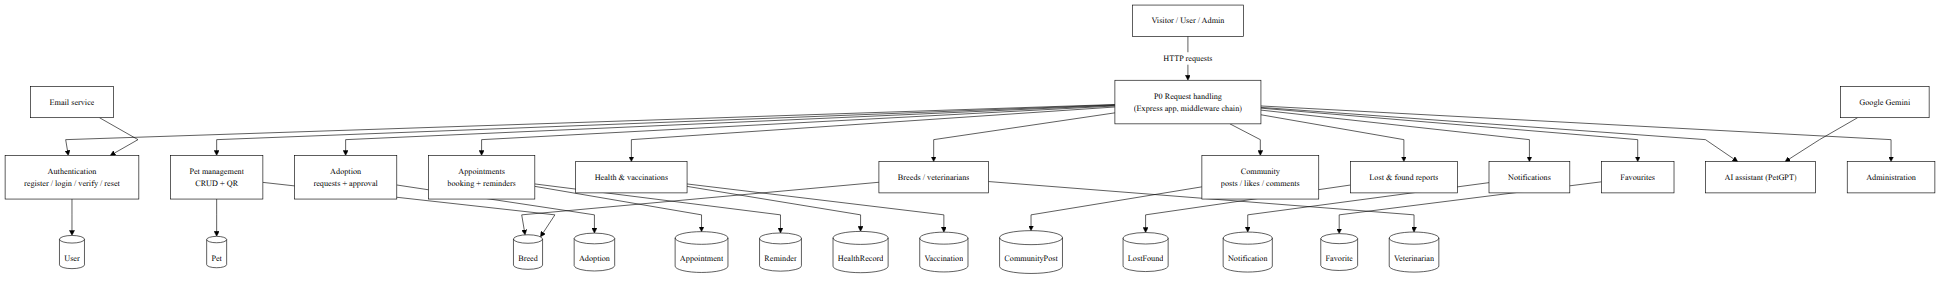
\includegraphics[width=\textwidth]{figures/03-dataflow.png}
    \caption{Top-level data-flow diagram of the FamiPet backend.}
    \label{fig:dataflow}
\end{figure}

The data-flow diagram groups the processes by the route modules that expose them
and shows the single store, MongoDB, with which every process interacts. Two
external data sinks are visible: the e-mail service, written to only by the
authentication process, and the AI service, which is reached by the AI process
and the Google Gemini endpoint.

In practice each subsystem respects the same flow, e.g. an appointment booking
produces a request on \texttt{POST /api/appointments}, and the controller writes
an \texttt{Appointment} document, synchronously creates a \texttt{Notification}
document and a \texttt{Reminder} document, and then responds with the created
record. This flow is the reason the application requires no background workers:
all derived records (notifications, reminders) are created at request time, in
the same transaction context provided by the database connection.

\section{Technology Stack}

The table below lists the technologies verified in the project implementation and
how each is used.

\begin{center}
\begin{longtable}{@{}p{3.4cm}p{3.0cm}p{8.1cm}@{}}
\toprule
\textbf{Technology} & \textbf{Type} & \textbf{How it is used} \\
\midrule
Node.js & Runtime & Executes the backend (\texttt{server.js}) on a single
process, port 5000 by default. \\
Express 4 & Web framework & Routing, JSON bodies (50\,MB limit), static files,
URL-encoded bodies, final error and 404 handlers. \\
MongoDB & Database & Persistent document store (\texttt{animal\_planet} by
default). \\
Mongoose 8 & ODM & 13 models mapped to collections; schema validation, enum
constraints, unique compound indexes, pre-save hashing hooks, query methods. \\
jsonwebtoken & Auth & Signs and verifies the bearer JWT with a 30-day expiry by
default. \\
bcryptjs & Auth & Hashes passwords with cost factor 12 and compares them on
login. \\
crypto & Auth & Generates 32-byte random tokens, hashed with SHA-256 before
storage, for e-mail verification and password reset. \\
nodemailer & E-mail & Sends HTML e-mails through SMTP (Gmail service by default). \\
multer & Upload & Accepts image uploads (JPEG/PNG/WebP, max 5\,MB) to the
\texttt{uploads/} directory. \\
qrcode & QR & Generates a PNG data-URL QR code for the digital pet identity. \\
cloudinary & Images & Optional image-hosting integration read from environment
configuration. \\
@google/generative-ai & AI & Defines the Gemini model, but the implementation
calls the REST endpoint directly with \texttt{fetch}. \\
morgan & HTTP logging & Development request logging. \\
compression & HTTP & GZIP-style response compression. \\
helmet & Security & Sets security HTTP headers, with
cross-origin-resource policy relaxed so uploaded images render on the frontend
origin (Section~\ref{sec:security}). \\
cors & Security & Origin-guard that permits the configured client origin,
localhost, and private LAN ranges. \\
node-cron & Declared & Declared but unused; no scheduled jobs exist. \\
socket.io & Declared & Declared but unused; no real-time channel exists. \\
React + TypeScript & Frontend & The in-progress migration stack used by
\texttt{frontend-react}. \\
Vite + Tailwind CSS & Frontend tooling & Build tooling and styling for the React
migration. \\
\bottomrule
\end{longtable}
\end{center}

\section{Analysis of Design Decision Consequences}

Two configuration observations are worth recording because they affect how the
system behaves at runtime.

First, the PetGPT assistant is implemented against Google's Gemini REST endpoint
(system instruction, contents, 25-second timeout, and a keyword fallback). The
OpenAI \texttt{PETGPT\_OPENAI\_*} variables in \texttt{backend/.env.example} are
not implemented, so the active provider is always Google when a key is present.
Second, reminders are not pushed asynchronously: the \texttt{Reminder}
collection records date and time, but no background scheduler delivers
notifications; the reminders are presented to the user through the reminders
API. Both facts are documented here so the reader does not mistake declared
dependencies for delivered behaviour.
\famichapter{System Architecture and Design}{This chapter describes the logical
architecture of FamiPet, the request lifecycle, the deployment layout, and the
responsibility of each component.}{ch:arch}

\section{Architecture Style}

FamiPet is a client--server application whose backend is a \emph{modular
monolith}: one Express process exposes all sixteen route modules, and all
business logic, validation, and persistence live in that process against a single
MongoDB store. There are no microservices, no message broker, and no background
workers. This architecture was chosen because the functional requirements are
interdependent (appointments create reminders and notifications; adoption
approval updates the pet and notifies the applicant) and the data is shared, so a
single transaction context keeps the flows simple, consistent, and testable.

Figure~\ref{fig:layered} shows the layered structure of the backend as it is
implemented. The presentation boundary is the HTTP API consumed by the web
client. Gateway middleware sets the security and parsing context. The routing
layer maps the sixteen route modules, and access-control middleware
(\texttt{protect}, \texttt{adminOnly}, \texttt{upload}) enforces identity,
roles, and file constraints. The controller layer implements the business logic.
The data layer maps the 13 Mongoose models to MongoDB collections. Two external
boundaries are drawn: e-mail and AI.

\begin{figure}[htbp]
    \centering
    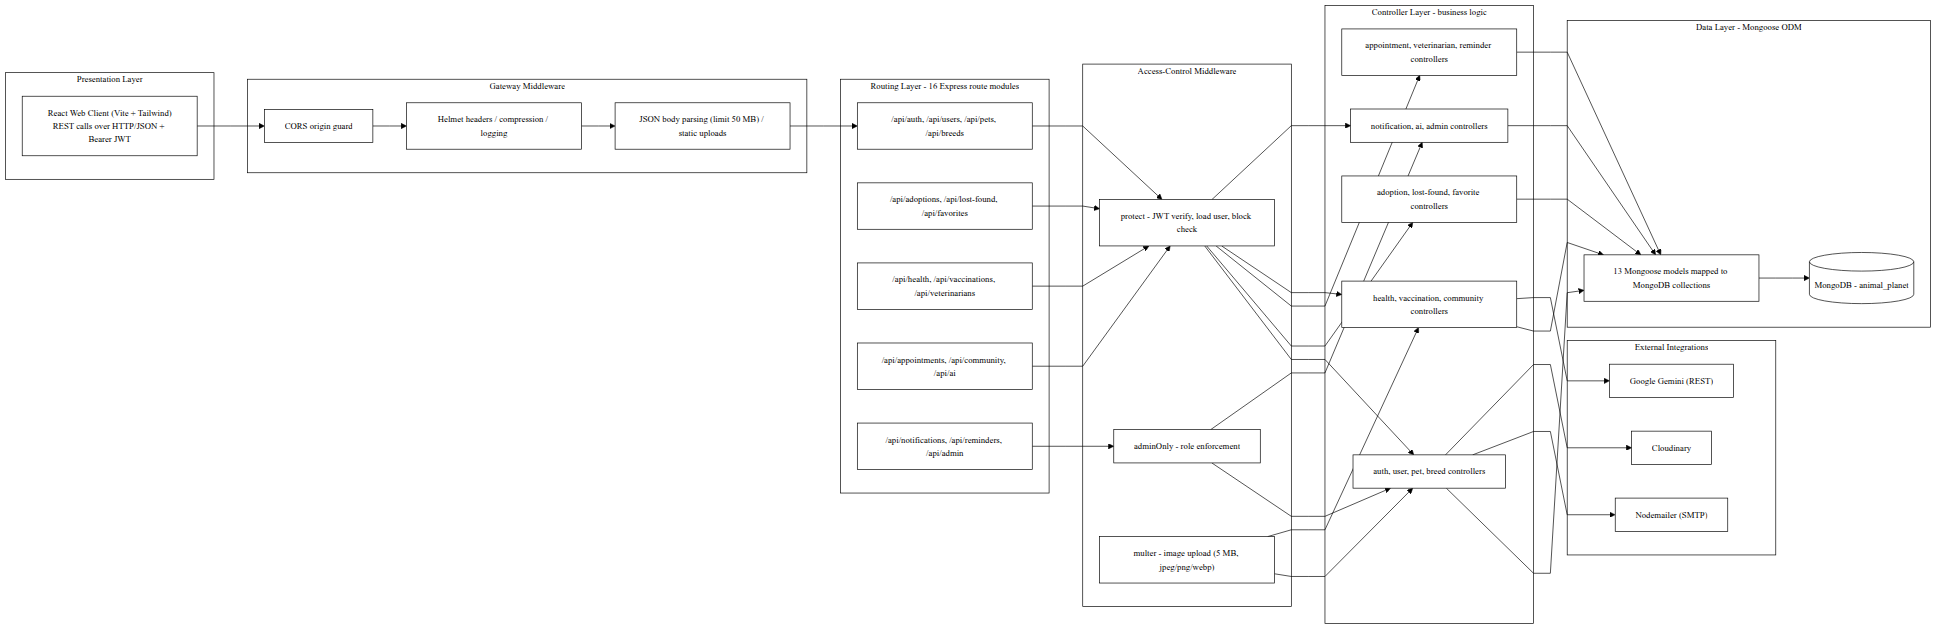
\includegraphics[width=\textwidth]{figures/04-layered-arch.png}
    \caption{Layered architecture of the FamiPet backend.}
    \label{fig:layered}
\end{figure}

The layered diagram reflects the actual module boundaries of the repository.
Cross-cutting concerns (CORS, helmet, compression, JSON parsing) run before any
route module. The \texttt{protect} middleware runs on every protected route, the
\texttt{adminOnly} middleware on administrative routes, and the
Multer~\cite{multer} upload
middleware only on routes that accept images.

\section{Module Responsibilities}

The table below lists the sixteen Express route modules and the central
responsibilities of their controllers.

\begin{center}
\begin{longtable}{@{}p{3.6cm}p{11.0cm}@{}}
\caption{Backend route modules and responsibilities.}
\label{tab:modules}\\
\toprule
\textbf{Route module} & \textbf{Responsibility} \\
\midrule
\path{/api/auth} & Register, verify and resend e-mail verification, login,
forgot/reset password, current user, profile update, password change. \\
\path{/api/users} & Public user lookup, favorites toggle, avatar upload. \\
\path{/api/pets} & Public pet listing, featured pets, own pets, pet CRUD with
owner enforcement, QR generation. \\
\path{/api/breeds} & Public breed catalogue; admin create/update/delete. \\
\path{/api/adoptions} & Adoption applications, own applications, admin listing
and status updates with pet transition and notification. \\
\path{/api/lost-found} & Public reports, owner CRUD, admin status updates and
deletion. \\
\path{/api/health} & Owner-scoped health records per pet. \\
\path{/api/vaccinations} & Owner-scoped vaccination records and upcoming list. \\
\path{/api/favorites} & Owner-scoped favourite pets (unique user--pet pairs). \\
\path{/api/veterinarians} & Public directory; admin CRUD. \\
\path{/api/appointments} & Booking with slot conflict check, auto-notification
and auto-reminder, reschedule and cancel with reminder sync. \\
\path{/api/community} & Public posts, owner CRUD, likes, comments; admin
moderation. \\
\path{/api/ai} & \texttt{/ask} (PetGPT over Gemini with fallback) and
\texttt{/advice} (rule-based per-pet advice). \\
\path{/api/notifications} & Owner-scoped notification read, unread, mark
read/all-read, delete. \\
\path{/api/reminders} & Owner-scoped reminders CRUD and completion. \\
\path{/api/admin} & Dashboard statistics, user/pet/lost-found/community
administration. \\
\bottomrule
\end{longtable}
\end{center}

\section{Request Lifecycle}

Figure~\ref{fig:lifecycle} shows the lifecycle of a protected request, using the
example of an authenticated controller that owns a resource. The sequence is
identical for every protected subsystem; the ownership predicate is the only
part that varies (see Chapter~\ref{ch:auth}).

\begin{figure}[htbp]
    \centering
    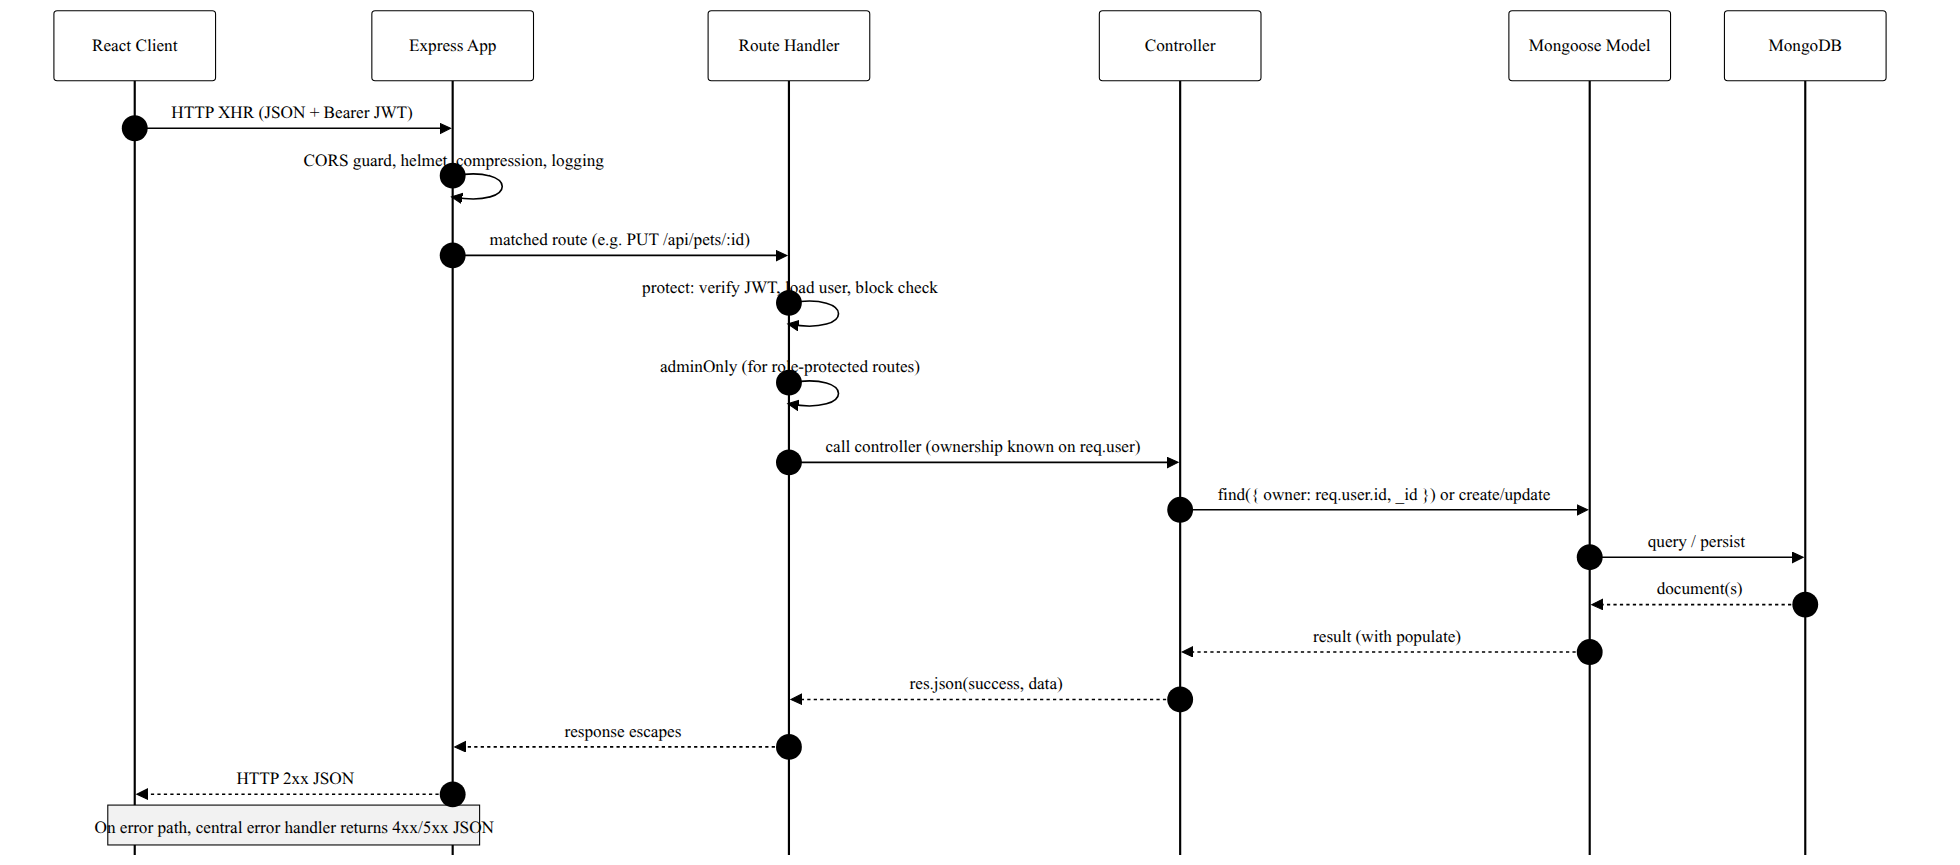
\includegraphics[width=\textwidth]{figures/06-request-lifecycle.png}
    \caption{Lifecycle of a protected request through the backend.}
    \label{fig:lifecycle}
\end{figure}

Once the token is verified and the user is loaded, owner-scoped queries bind the
resource to \texttt{req.user.\_id}: for example, appointments are queried with
\texttt{\{user: req.user.\_id\}}, health records and vaccinations the same way,
and pet operations compare \texttt{pet.owner} to \texttt{req.user.id}. This
binding is what makes user isolation enforceable without trusting any
client-supplied identifier.

\section{Deployment}

Figure~\ref{fig:deploy} shows the deployment layout used during the project. The
backend process and the frontend are served on different ports; the database
runs as a separate service, optionally with local tooling (Compass) for
inspection. The backend also serves the \texttt{uploads} directory statically so
uploaded images resolve from the API. Credentials for the optional external
image-hosting platform Cloudinary~\cite{cloudinary} are declared in the
configuration but the current implementation stores uploads locally on disk.

\begin{figure}[htbp]
    \centering
    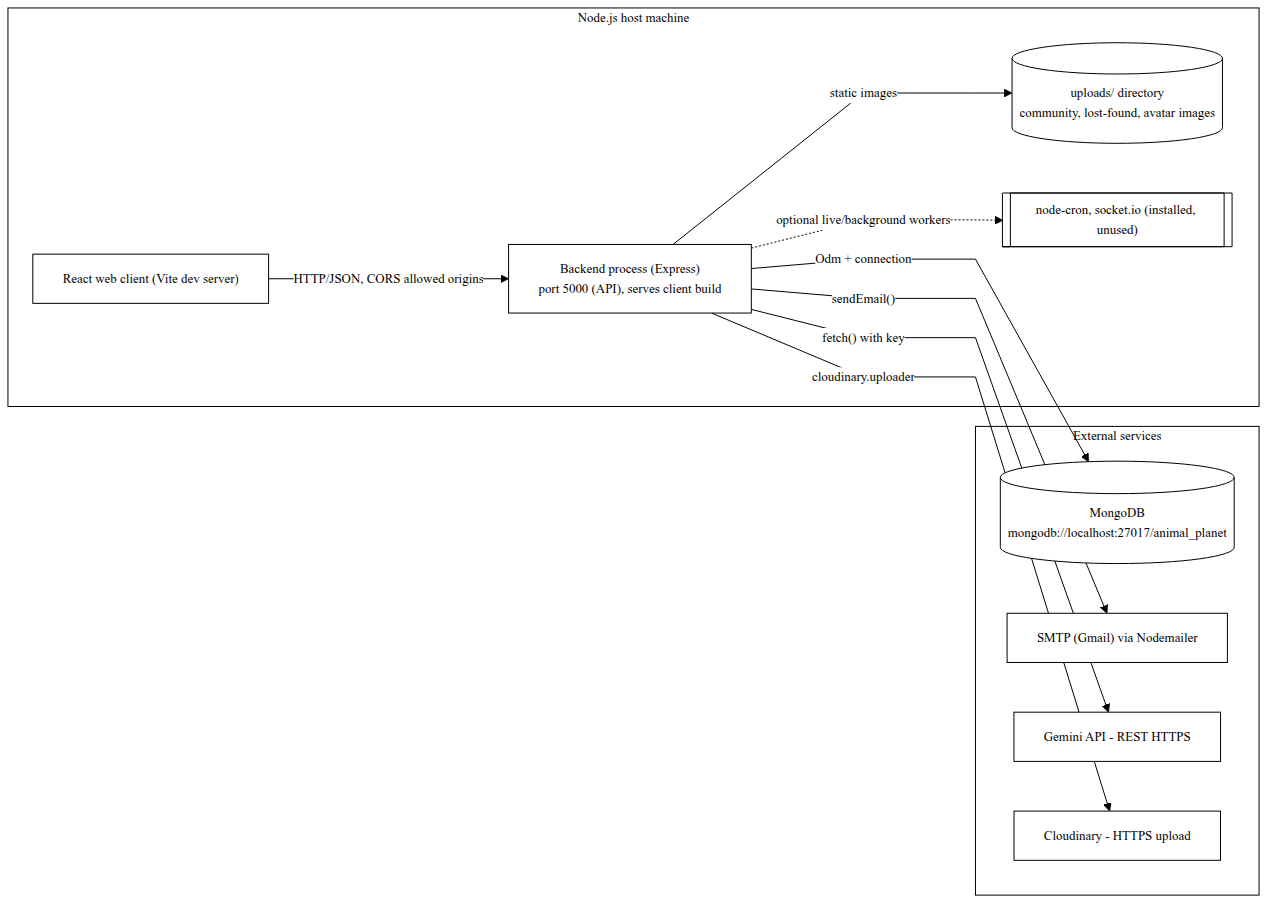
\includegraphics[width=\textwidth]{figures/07-deployment.png}
    \caption{Deployment layout of FamiPet.}
    \label{fig:deploy}
\end{figure}

The server binds to the environment-configured port (5000 by default). The
client origin is taken from \texttt{CLIENT\_URL} (5000-series Live Server/Vite by
default) and is also used to fall back to a locally served page for the
verify-email and reset-password routes. MongoDB connects through
\path{MONGODB\_URI}, defaulting to
\path{mongodb://localhost:27017/animal\_planet}.
\famichapter{Data Management and Data Model}{This chapter documents the MongoDB
data model: the thirteen entities, their relationships, and the constraints and
indexes that protect data integrity.}{ch:data}

\section{Database Design}

FamiPet uses MongoDB~\cite{mongodb} as its primary store. The schema is defined
in thirteen Mongoose~\cite{mongoose} models, all located in \texttt{backend/models/}. Figure~\ref{fig:er}
shows the entity--relationship view of the store. Dashed lines mark references
whose target documents are populated through Mongoose \texttt{populate}.

\begin{figure}[p]
    \centering
    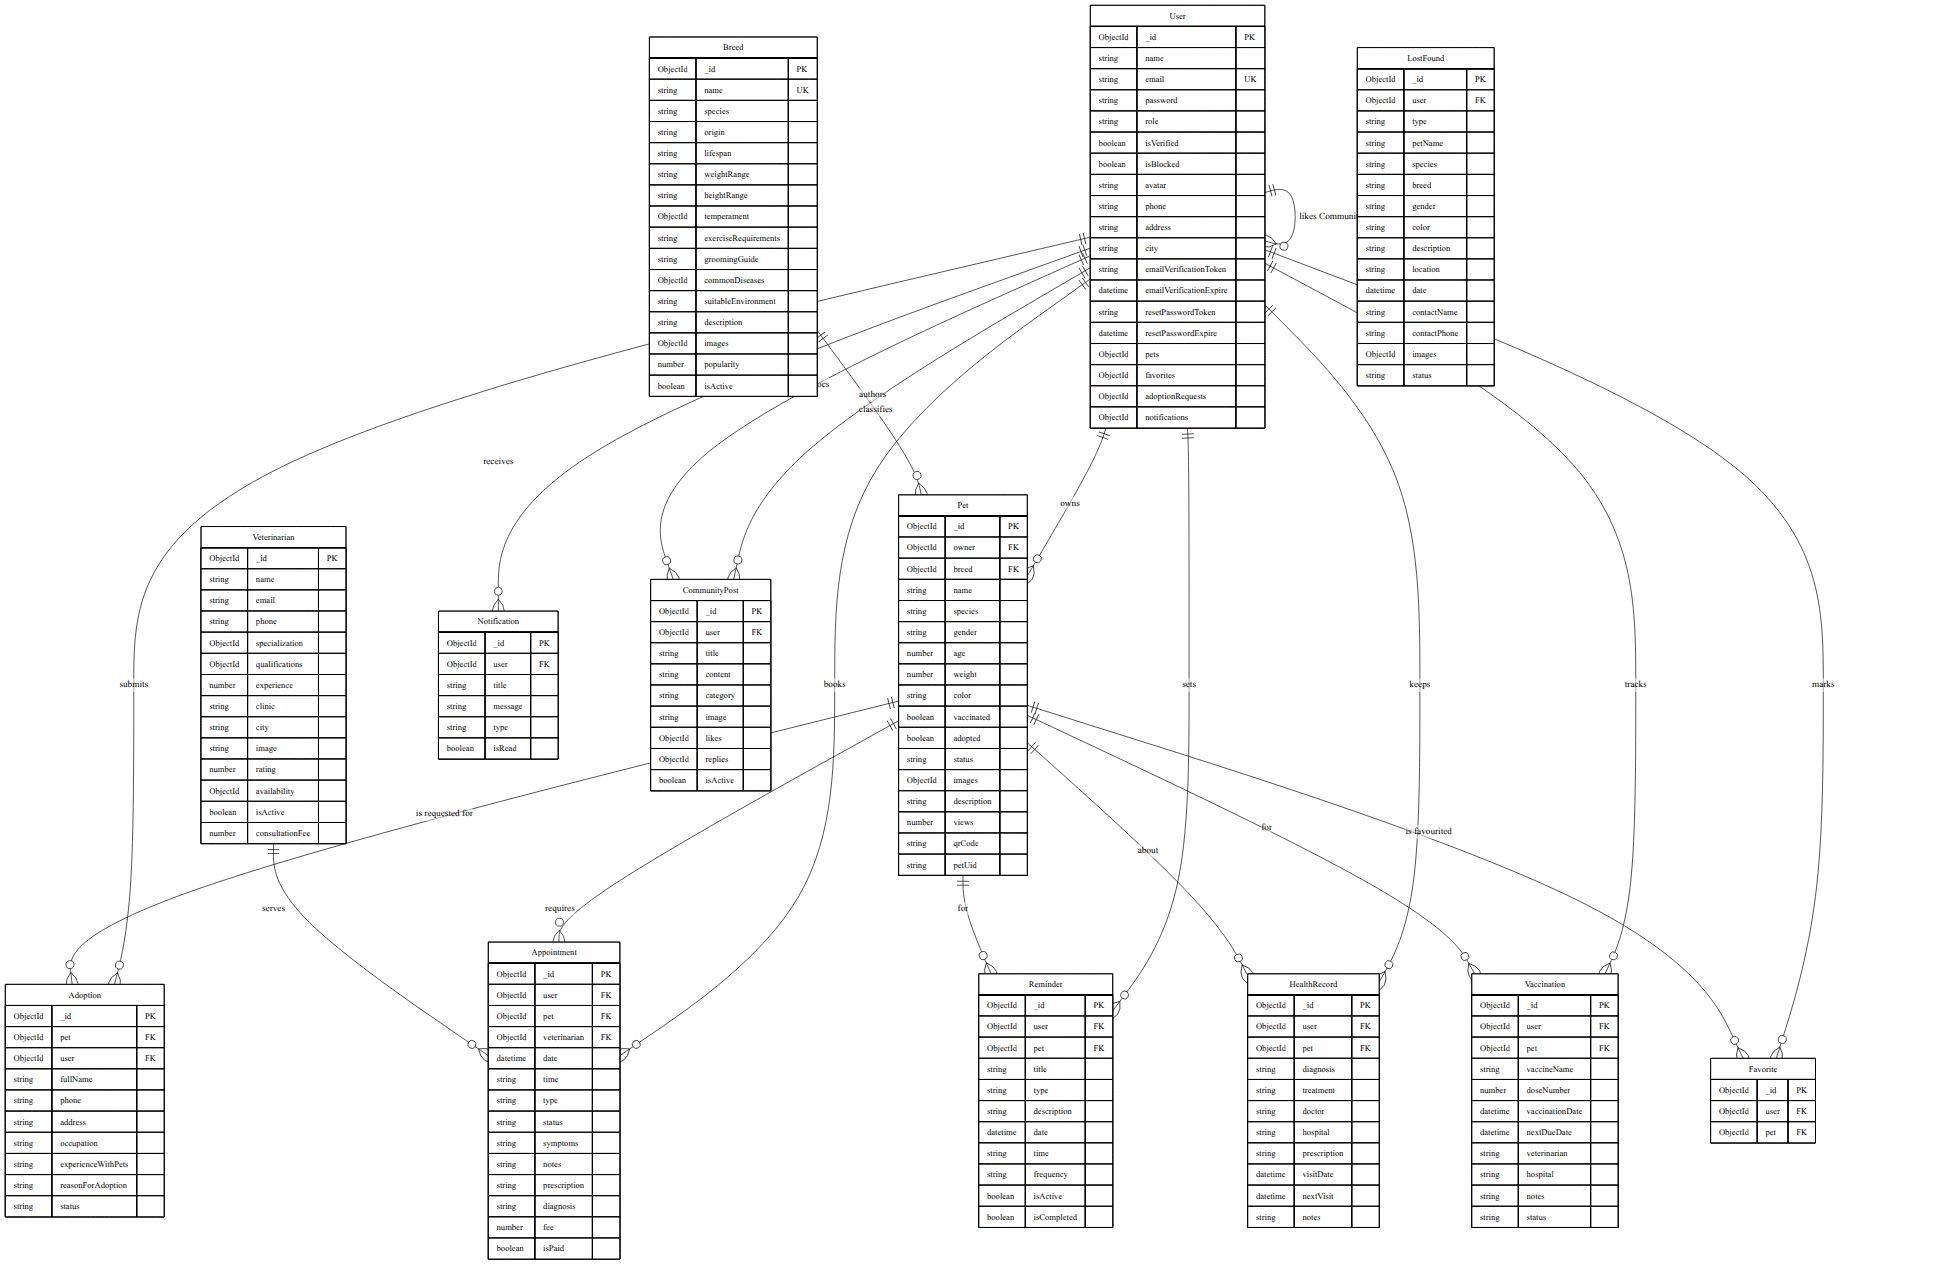
\includegraphics[width=\textwidth]{figures/08-er-diagram.png}
    \caption{Entity--relationship diagram of the FamiPet database.}
    \label{fig:er}
\end{figure}

The central entity is \texttt{Pet}. Every pet belongs to exactly one
\texttt{User} (the \texttt{owner}) and references exactly one \texttt{Breed}.
Users may star pets through \texttt{Favorite}, whose compound unique index
guarantees that the same user cannot favourite the same pet twice. Health
records and vaccinations belong to a user and a pet, appointments to a user, a
pet, and a veterinarian, and reminders to a user with an optional pet reference.
Adoption requests belong to a user and a pet, and their status is managed by
administrators. Community posts embed arrays of likes and comments; lost-and-found
reports record animal and contact information. Notifications are per-user
documents that record read state.

\section{Entities and Collections}

\begin{center}
\begin{longtable}{@{}p{3.0cm}p{3.3cm}p{8.3cm}@{}}
\caption{Mongoose models and collections.}
\label{tab:models}\\
\toprule
\textbf{Model} & \textbf{Collection} & \textbf{Key fields} \\
\midrule
User & \texttt{users} & name, email (unique), password (select false), avatar,
phone, address, city, role (user/admin), isVerified, isBlocked,
emailVerificationToken + expire (SHA-256), resetPasswordToken + expire
(SHA-256), pets[], favorites[], adoptionRequests[], notifications[]. \\
Pet & \texttt{pets} & owner, breed, name, species (dog/cat/bird/rabbit/fish/
other), gender, age, weight, color, vaccinated, adopted, status
(available/adopted/lost/inactive), images[], description, views, qrCode,
petUid. \\
Breed & \texttt{breeds} & name (unique), species, origin, lifespan, weight/
height range, temperament[], exerciseRequirements, groomingGuide,
commonDiseases[], suitableEnvironment, description, images[], popularity,
isActive. \\
Adoption & \texttt{adoptions} & pet, user, fullName, phone, address, occupation,
experienceWithPets, reasonForAdoption, status (Pending/Approved/Rejected). \\
Appointment & \texttt{appointments} & user, pet, veterinarian, date, time, type
(\path{checkup/vaccination/surgery/emergency/grooming/consultation}), status
(\path{pending/confirmed/completed/cancelled/no-show}), symptoms, notes,
prescription, diagnosis, fee, isPaid. \\
Notification & \texttt{notifications} & user, title, message, type
(\path{adoption/appointment/vaccination/health/system/other}), isRead. \\
Reminder & \texttt{reminders} & user, pet, title, type (feeding/medicine/
vaccination/grooming/appointment/exercise/custom), description, date, time,
frequency (once/daily/weekly/monthly), isActive, isCompleted. \\
HealthRecord & \texttt{healthrecords} & user, pet, diagnosis, treatment, doctor,
hospital, prescription, visitDate, nextVisit, notes. \\
Vaccination & \texttt{vaccinations} & user, pet, vaccineName, doseNumber,
vaccinationDate, nextDueDate, veterinarian, hospital, notes, status
(Pending/Completed). \\
Favorite & \texttt{favorites} & user, pet, with a unique compound index. \\
Veterinarian & \texttt{veterinarians} & name, email, phone, specialization[],
qualifications[], experience, clinic, address, city, image, rating, reviews[],
availability[], isActive, consultationFee. \\
CommunityPost & \texttt{communityposts} & user, title, content, category, image,
likes[], comments[] (embedded), isActive. \\
LostFound & \texttt{lostfounds} & user, type (lost/found), petName, species,
breed, gender, color, description, location, date, contactName, contactPhone,
images[], status (active/resolved). \\
\bottomrule
\end{longtable}
\end{center}

\section{Constraints and Indexes}

The schema enforces integrity at three levels.

\begin{itemize}
    \item \textbf{Required and enum constraints.} Required fields are declared in
    each schema, and enumerated fields (\texttt{role}, \texttt{species},
    \texttt{status}, message and reminder types, appointment type and status,
    adoption status) are constrained to the documented values. Violations
    surface as Mongoose \texttt{ValidationError}s and are returned as HTTP 400.
    \item \textbf{Unique indexes.} \texttt{User.email} is unique;
    \texttt{Breed.name} is unique; \texttt{Favorite} carries a compound unique
    index on \texttt{\{user, pet\}} that prevents duplicate favourites. Duplicate
    key violations (error code 11000) are mapped to HTTP 400 by the error
    handler.
    \item \textbf{Pre-save hooks.} The \texttt{User} schema hooks \texttt{save}
    and hashes the password with bcrypt (cost factor 12) whenever the password
    field has been modified. The \texttt{password} field uses \texttt{select:
    false} so it is excluded from all queries unless the controller explicitly
    selects it (login, change-password, reset flows).
\end{itemize}

\section{Relationship Coverage Between Models}

The ER diagram and the entity table together demonstrate that every
user-specific document carries the owning user reference and is queried with
that reference. This pattern is the data-level backbone of the access control
described in Chapter~\ref{ch:auth}: a record created by user A is stored with
\texttt{user: A}, so every later owner-scoped query naturally excludes user\,B's
data even before any authorization logic runs.
\famichapter{Authentication, Authorization, and Security}{This chapter explains
how FamiPet establishes user identity, how it enforces authorization, and the
security controls applied at the HTTP and storage layers.}{ch:auth}

\section{Content}
\label{sec:authoverview}

Authentication is handled entirely by the backend. The flow has three stages:
account creation with e-mail verification, login with a signed token, and
token-based access control for every protected route. Figures~\ref{fig:reg}
through~\ref{fig:reset} show the four authentication workflows as implemented.

\subsection{Registration and E-mail Verification}

\begin{figure}[htbp]
    \centering
    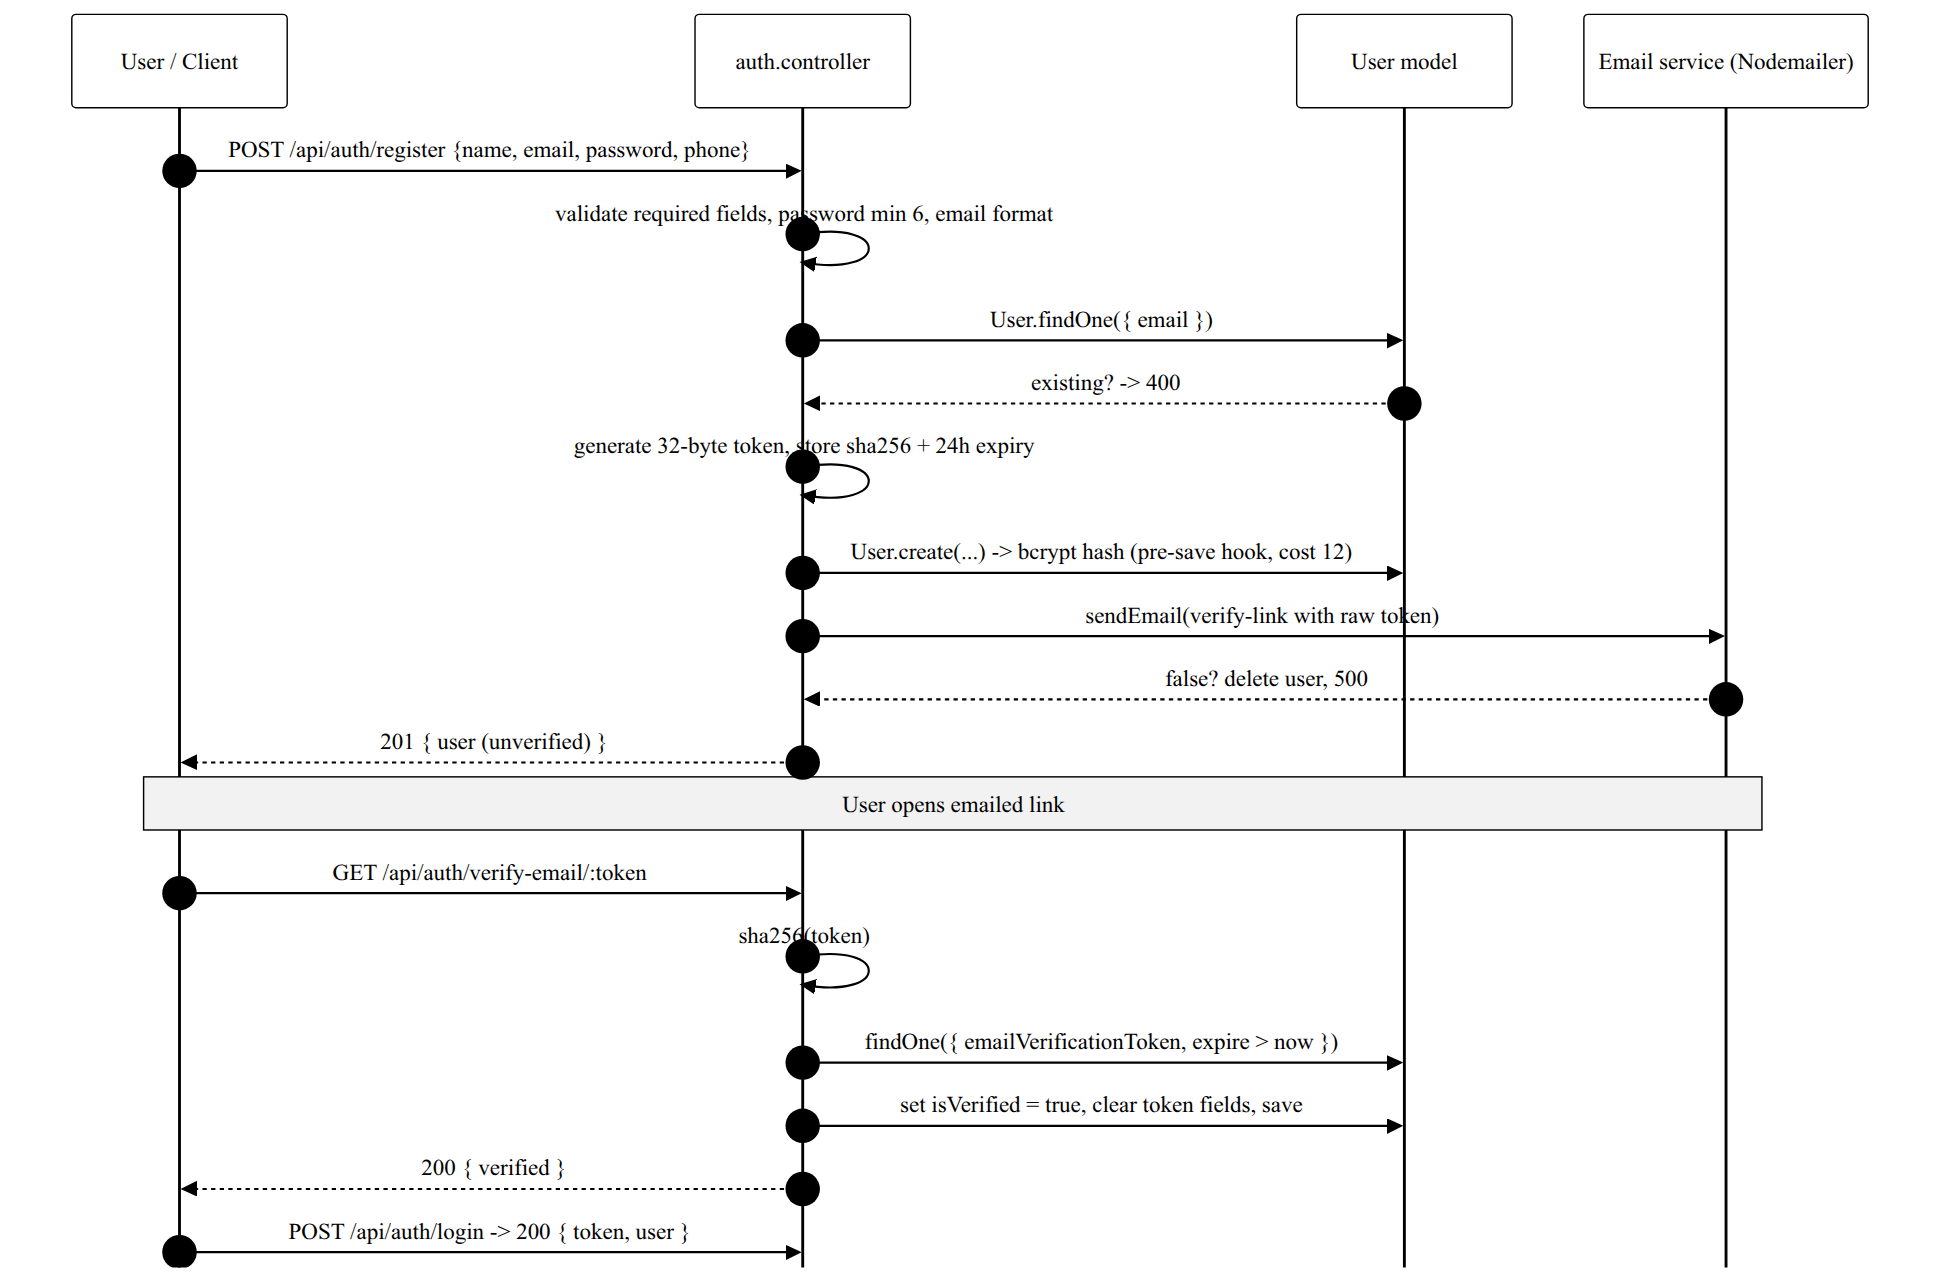
\includegraphics[width=\textwidth]{figures/09-register-verify.png}
    \caption{Registration and e-mail verification flow.}
    \label{fig:reg}
\end{figure}

When \texttt{POST /api/auth/register} is received, the controller validates the
fields, normalizes the e-mail, checks whether it already exists, generates a
32-byte verification token, stores only its SHA-256 hash with a 24-hour expiry,
hashes the password through the pre-save hook, and creates the user with
\texttt{isVerified: false}. An HTML e-mail containing a verification link is
sent through Nodemailer; if the e-mail cannot be sent the user document is
deleted so no unverifiable account remains. Clicking the link calls
\texttt{GET /api/auth/verify-email/:token}, which hashes the presented token and
marks the user verified. A resend endpoint generates a fresh token for
unverified accounts. Login is refused for unverified accounts
(HTTP 403, \texttt{isVerified: false} in the response).

\subsection{Login and Token Issuance}

\begin{figure}[htbp]
    \centering
    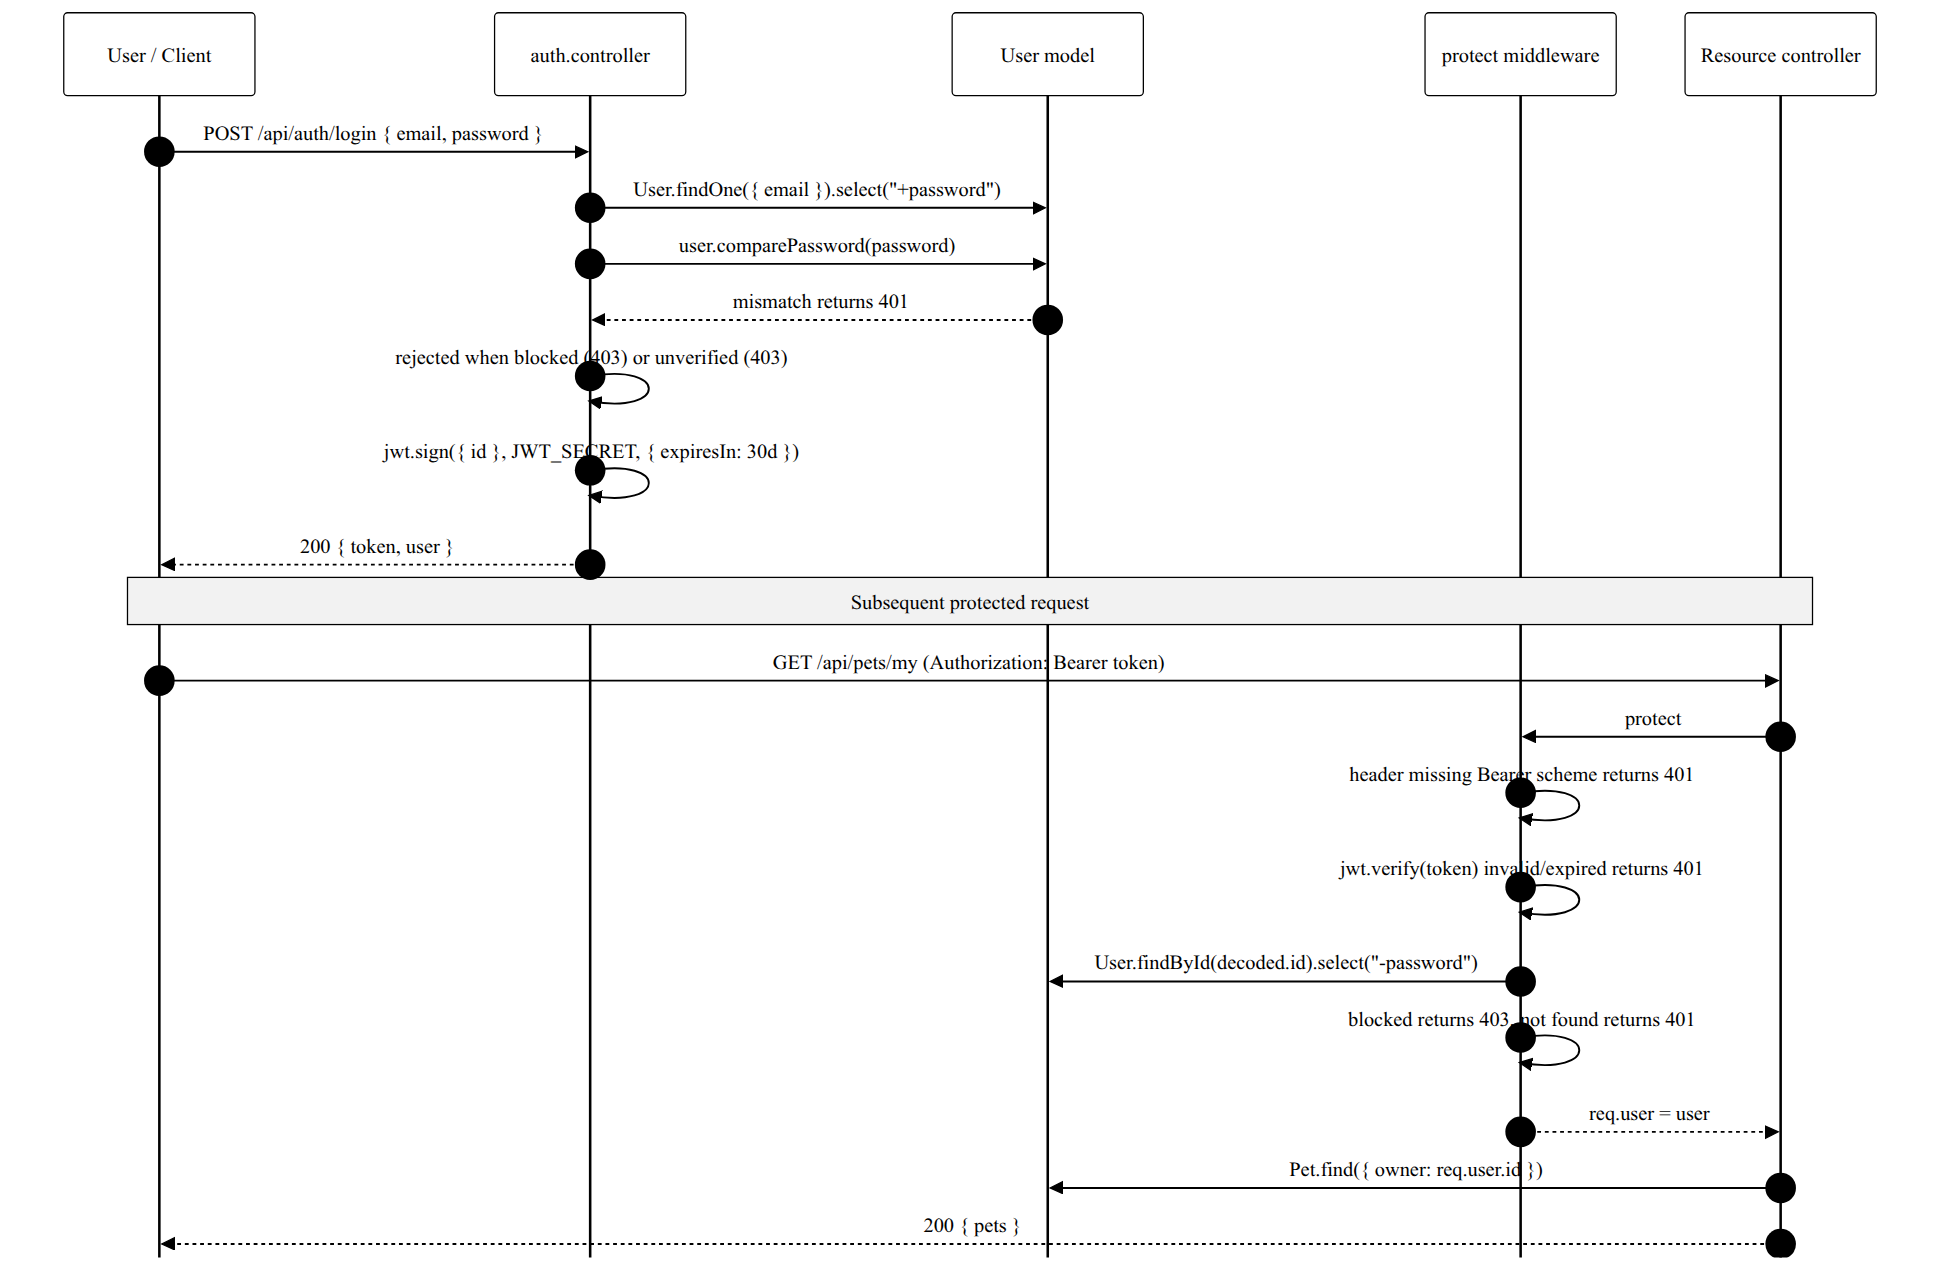
\includegraphics[width=\textwidth]{figures/10-login-token.png}
    \caption{Login and JWT issuance flow.}
    \label{fig:login}
\end{figure}

\texttt{POST /api/auth/login} selects the user including the (normally excluded)
password, compares the presented password with the stored bcrypt hash, refuses
blocked and unverified accounts, and on success signs a JWT containing the user
identifier with the configured secret and a 30-day expiry (\texttt{JWT\_EXPIRE}).
The client stores the token and sends it as a bearer header on protected calls.
The \texttt{/api/auth/me} endpoint returns the current user with pets and
favourites populated.

\subsection{Token Verification and Role-Based Access}

Every protected route is wrapped by the \texttt{protect} middleware
(\texttt{backend/middleware/auth.js}). Figure~\ref{fig:access} shows its decision
tree.

\begin{figure}[htbp]
    \centering
    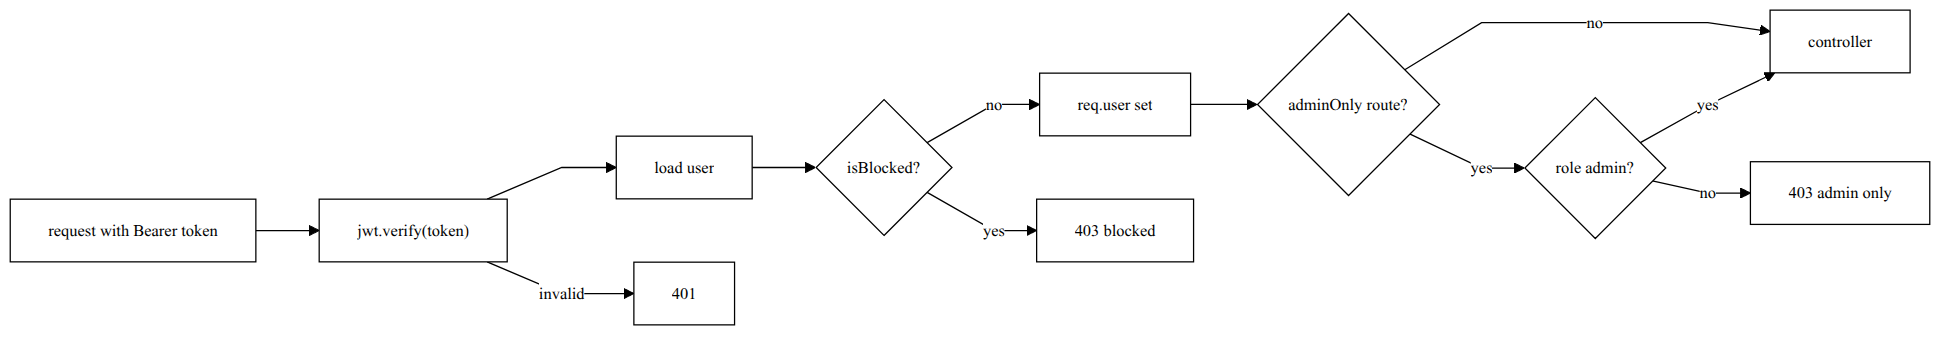
\includegraphics[width=\textwidth]{figures/11-access-control.png}
    \caption{Access-control decision tree (protect and adminOnly).}
    \label{fig:access}
\end{figure}

The middleware rejects requests without a bearer header (401), without a
configured \texttt{JWT\_SECRET} (500), with an invalid token (401), with a
missing user (401), or with a blocked account (403). On success it assigns
\texttt{req.user} from the database (excluding the password) and forwards the
request. The \texttt{adminOnly} middleware then enforces
\texttt{req.user.role === "admin"} for administrative routes, returning 403
otherwise. Ownership is applied separately inside the controllers: resources are
queried with the owner predicate and therefore return 404 for other users'
resources.

\subsection{Password Recovery}

\begin{figure}[htbp]
    \centering
    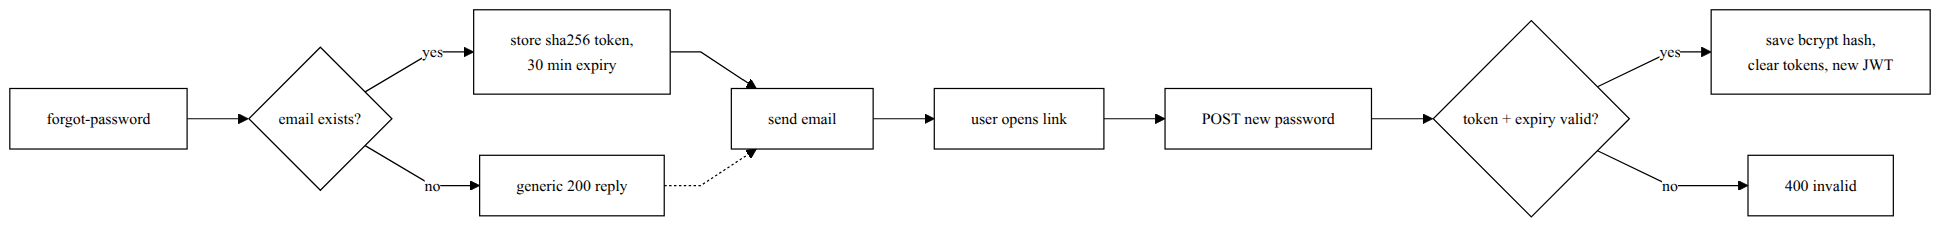
\includegraphics[width=\textwidth]{figures/12-password-reset.png}
    \caption{Password reset flow.}
    \label{fig:reset}
\end{figure}

\texttt{POST /api/auth/forgot-password} always returns a generic ``if the e-mail
is registered'' message so that the endpoint cannot be used to enumerate
accounts. A registered e-mail receives a link containing a 32-byte token; the
server stores only the SHA-256 hash with a 30-minute expiry. \texttt{POST
/api/auth/reset-password/:token} hashes the presented token, verifies it and the
expiry, stores the new password (bcrypt-hashed by the pre-save hook), clears the
token fields, and returns a fresh JWT so the user is logged in immediately. If
the e-mail cannot be delivered the stored token is cleared so a stale, unusable
token is not left on the account. A separate \texttt{change-password} endpoint
requires the current password.

\section{Security Controls}
\label{sec:security}

The security controls below are implemented and were verified in the Step 10
test campaign (Chapter~\ref{ch:testing}).

\begin{center}
\begin{longtable}{@{}p{3.6cm}p{11.0cm}@{}}
\toprule
\textbf{Control} & \textbf{Implementation} \\
\midrule
Password hashing & bcrypt cost 12 (\texttt{\$2a\$12\$} hashes verified directly
in the database). \\
Token hygiene & Verification and reset tokens are stored hashed (SHA-256);
plaintext tokens appear only in e-mail links. \\
JWT & Signed bearer tokens with \texttt{JWT\_SECRET}; invalid or expired tokens
yield 401. \\
E-mail verification gate & Unverified accounts cannot log in; forgot-password
does not reveal whether an e-mail exists. \\
Ownership isolation & All user-scoped queries bind to \texttt{req.user.\_id};
cross-user access to appointments, reminders, notifications, health records, and
vaccinations returns 404. \\
Role enforcement & \texttt{adminOnly} on all administrative routes; a regular
user receives 403. \\
Input validation & Backend-side checks for required fields, e-mail format,
password length, valid ObjectIds, real dates, ownership, and state transitions
returning 400/404/500. \\
CORS & Origin guard accepting the configured client, localhost, and private LAN
origins; preflight OPTIONS answered 204. \\
Security headers & Helmet headers with \texttt{crossOriginResourcePolicy:
cross-origin} so uploaded images are embeddable by the frontend origin. \\
Secret management & Keys live only in \texttt{backend/.env} (git-ignored);
only placeholder \texttt{.env.example} is committed; no secrets in repository
history. \\
Blocked accounts & \texttt{protect} and \texttt{login} reject blocked users with
403. \\
\bottomrule
\end{longtable}
\end{center}

\section{Security Boundary Verification}

The boundary behaviour was tested with two identities: a regular user and an
administrator. A regular user calling nine administrative endpoints
(\texttt{/api/admin/dashboard}, \texttt{/api/admin/users}, \texttt{/api/admin/
pets}, adoption listing and status update, \texttt{DELETE /api/admin/users/:id},
breed and veterinarian creation, and lost-and-found moderation) received 403 on
every call. A user attempting to read, update, or cancel another user's
appointment received 404 because the query is owner-scoped. These results are
recorded in the testing chapter (Chapter~\ref{ch:testing}).
\famichapter{Core Feature Implementation}{This chapter explains the core features
of FamiPet using their workflows, data, validation, and security behaviour, each
supported by a diagram.}{ch:features}

\section{Digital Pet Identity and QR Code}

\begin{figure}[htbp]
    \centering
    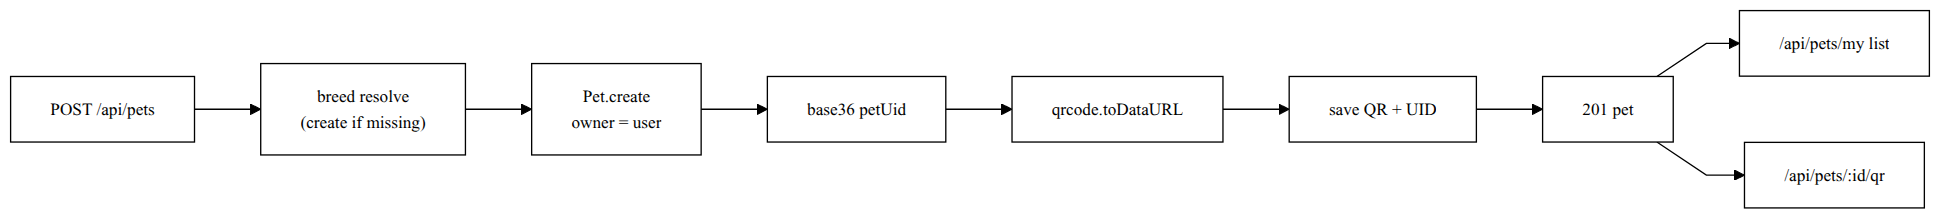
\includegraphics[width=\textwidth]{figures/13-pet-qr.png}
    \caption{Creation of a pet with automatic QR identity.}
    \label{fig:petqr}
\end{figure}

When a user creates a pet (\texttt{POST /api/pets}), the controller accepts
either a breed \texttt{ObjectId} or a breed name; a name is resolved to a breed
document and created on demand if absent. The pet is stored with
\texttt{owner: req.user.id}. A unique digital pet identifier is then generated
as \texttt{Date.now().toString(36)-petId.\allowbreak{}slice(-8)-random} and the
\texttt{qrcode} package encodes a JSON payload with the pet identifier, unique
ID, name, species, and breed into a PNG data URL that is persisted on the pet
document. The pet appears in the owner's list (\texttt{GET /api/pets/my}), and
the dedicated endpoint \texttt{GET /api/pets/:id/qr} regenerates a QR code whose
payload additionally includes the owner's public name and phone. The digital pet
identity is deliberately public-safe: the QR payload contains only identity and
public contact fields, never tokens, passwords, or the account reference
directly.

\section{Adoption Management}

\begin{figure}[htbp]
    \centering
    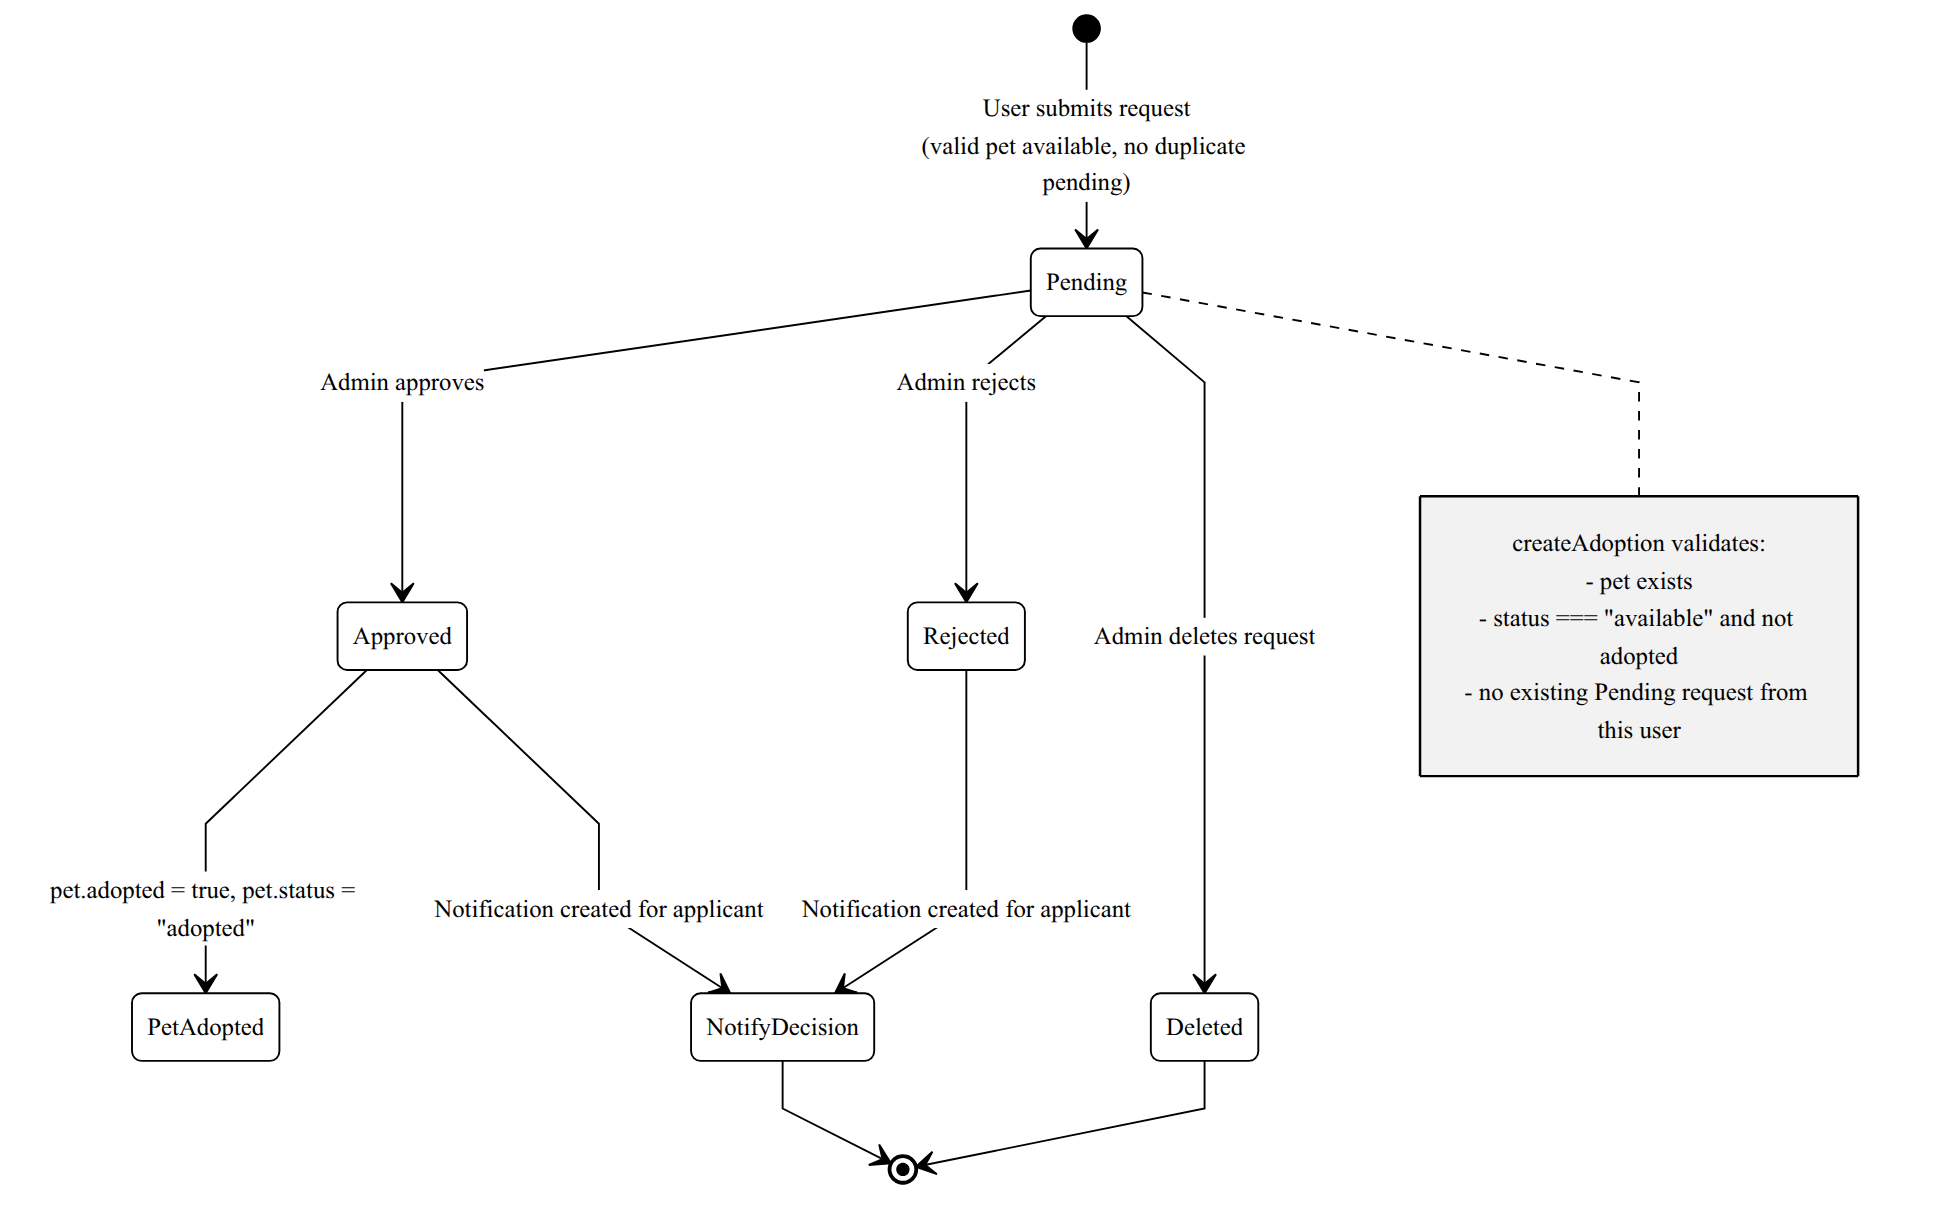
\includegraphics[width=\textwidth]{figures/14-adoption-state.png}
    \caption{Adoption request state diagram.}
    \label{fig:adoptstate}
\end{figure}

An adoption request (\texttt{POST /api/adoptions}) requires the pet reference,
full name, phone, address, and a reason. The controller verifies that the pet
exists, is \texttt{status: "available"} and not \texttt{adopted}, and that the
user has no already-pending request for the same pet; a duplicate is rejected.
The request is stored in the \texttt{Pending} state. Administrators transition
the state to \texttt{Approved} or \texttt{Rejected} through
\texttt{PUT /api/adoptions/:id} (admin-only). Approval automatically updates the
pet document (\texttt{adopted: true}, \texttt{status: "adopted"}), and every
status change creates a notification for the applicant with the pet's name and
the new state.

\begin{figure}[htbp]
    \centering
    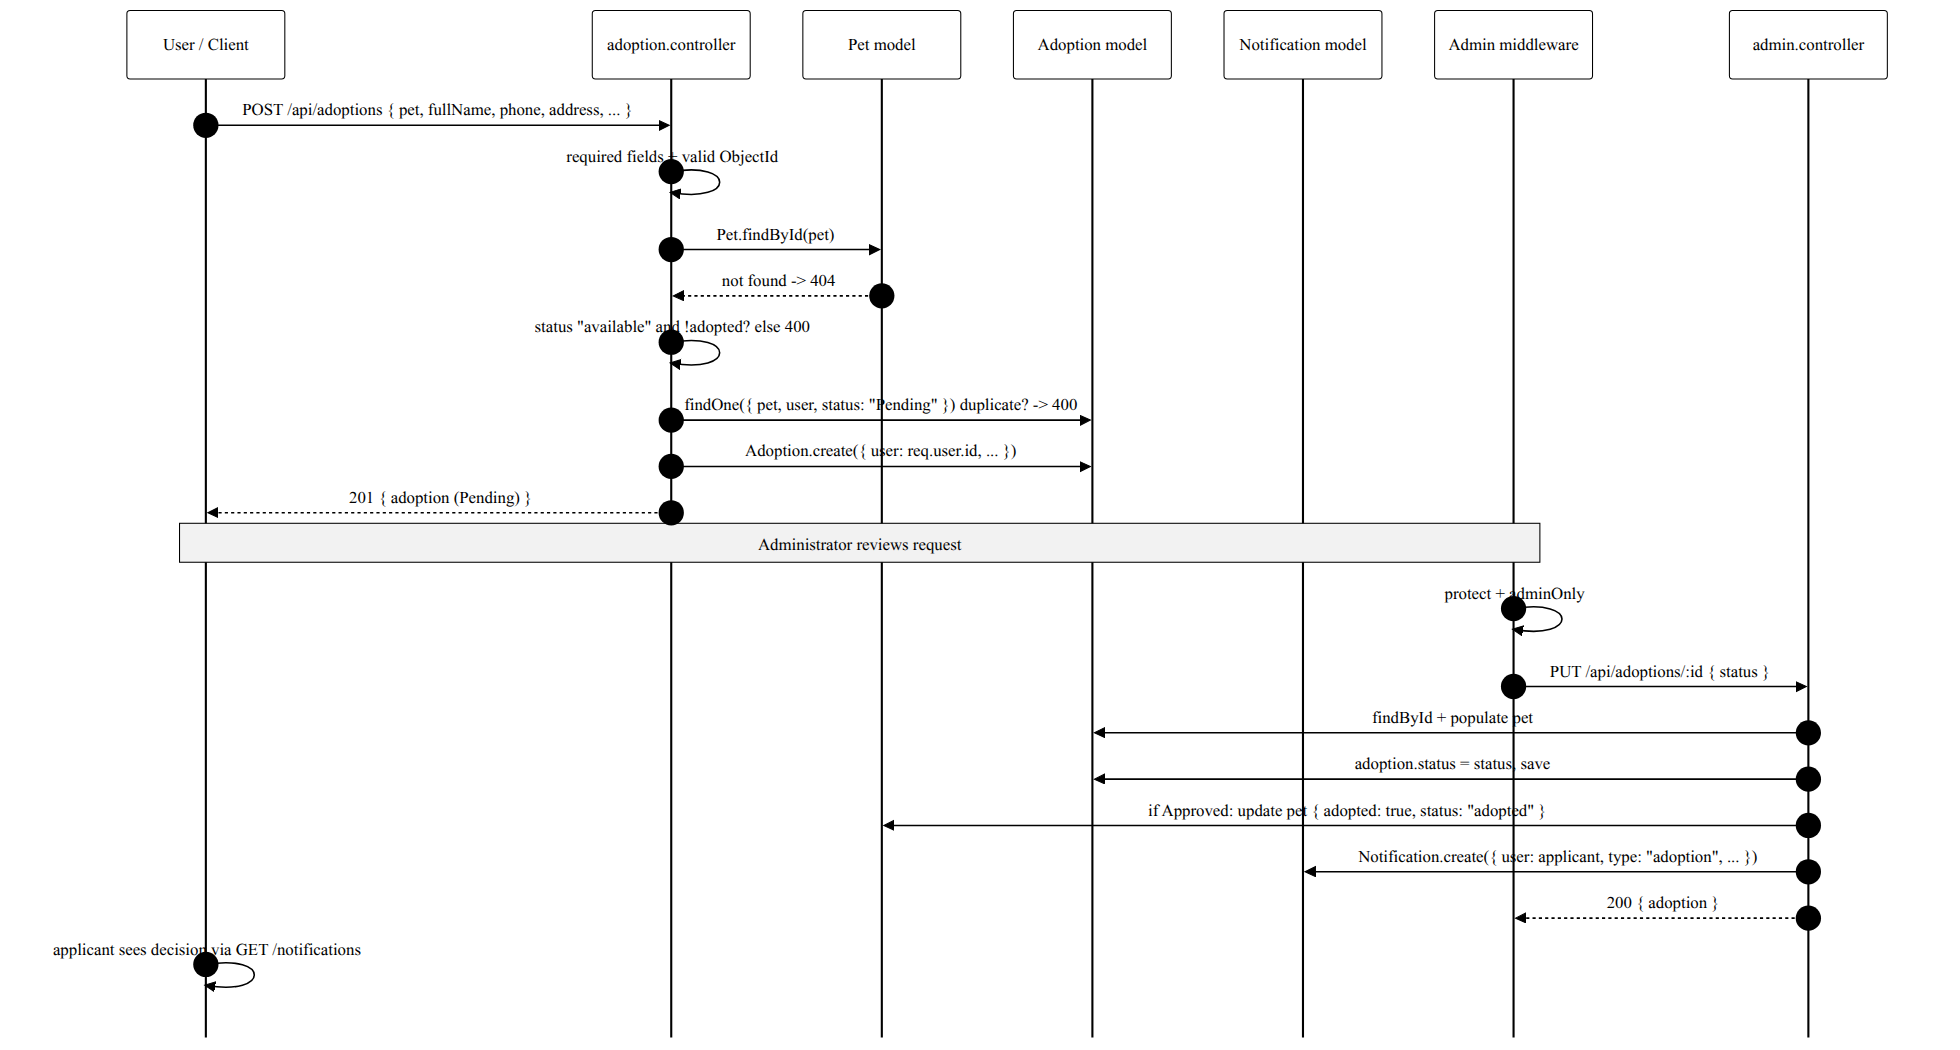
\includegraphics[width=\textwidth]{figures/15-adoption-sequence.png}
    \caption{Adoption application and approval sequence.}
    \label{fig:adoptseq}
\end{figure}

The sequence diagram shows the full path: the user submits the application, the
owners own pet records feed the adoption listing, the administrator reviews and
approves the request, the backend updates the pet and creates the applicant
notification, and the applicant reads both the updated request state and the
notification. Notification and pet-record data are stored in MongoDB, so both
survive a page reload.

\section{Appointments, Notifications, and Reminders}

Booking an appointment (\texttt{POST /api/appointments}) validates the pet and
veterinarian references, requires the pet to belong to the requesting user and
the veterinarian to be active, and rejects a double booking: an existing
appointment with the same veterinarian, date, and time in the
\texttt{pending} or \texttt{confirmed} state returns HTTP 400.

\begin{figure}[htbp]
    \centering
    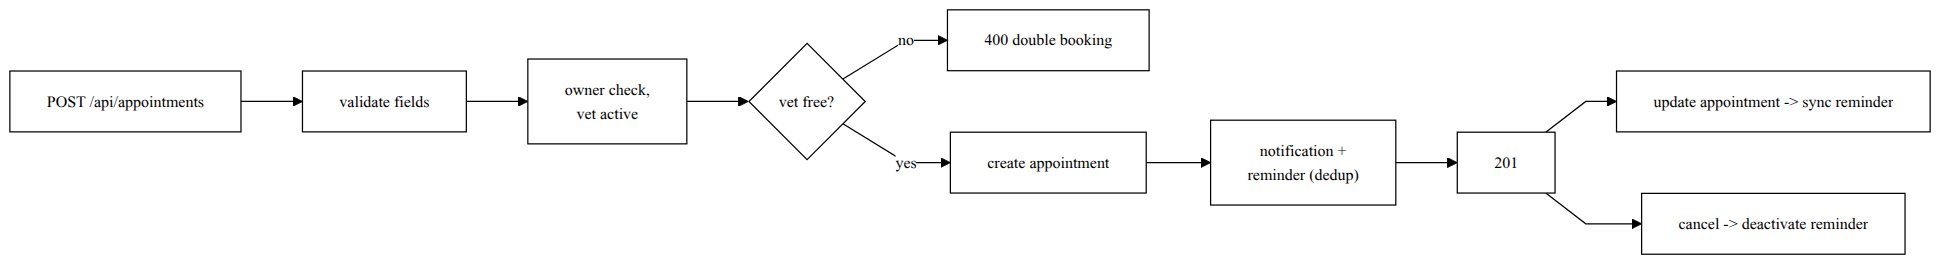
\includegraphics[width=\textwidth]{figures/16-appointment-flow.png}
    \caption{Appointment booking, rescheduling, and cancellation flow.}
    \label{fig:apptflow}
\end{figure}

On success the controller creates the appointment, immediately creates a
\texttt{Notification} (type \texttt{appointment}), and creates a
\texttt{Reminder} (type \texttt{appointment}, frequency \texttt{once}), but only
if an identical active reminder does not already exist, so repeat bookings do
not duplicate reminders. Rescheduling an appointment synchronizes the date and
time of the matching reminder; cancelling sets the appointment to
\texttt{cancelled} and deactivates the matching reminder so no stale active
reminder remains.

\begin{figure}[htbp]
    \centering
    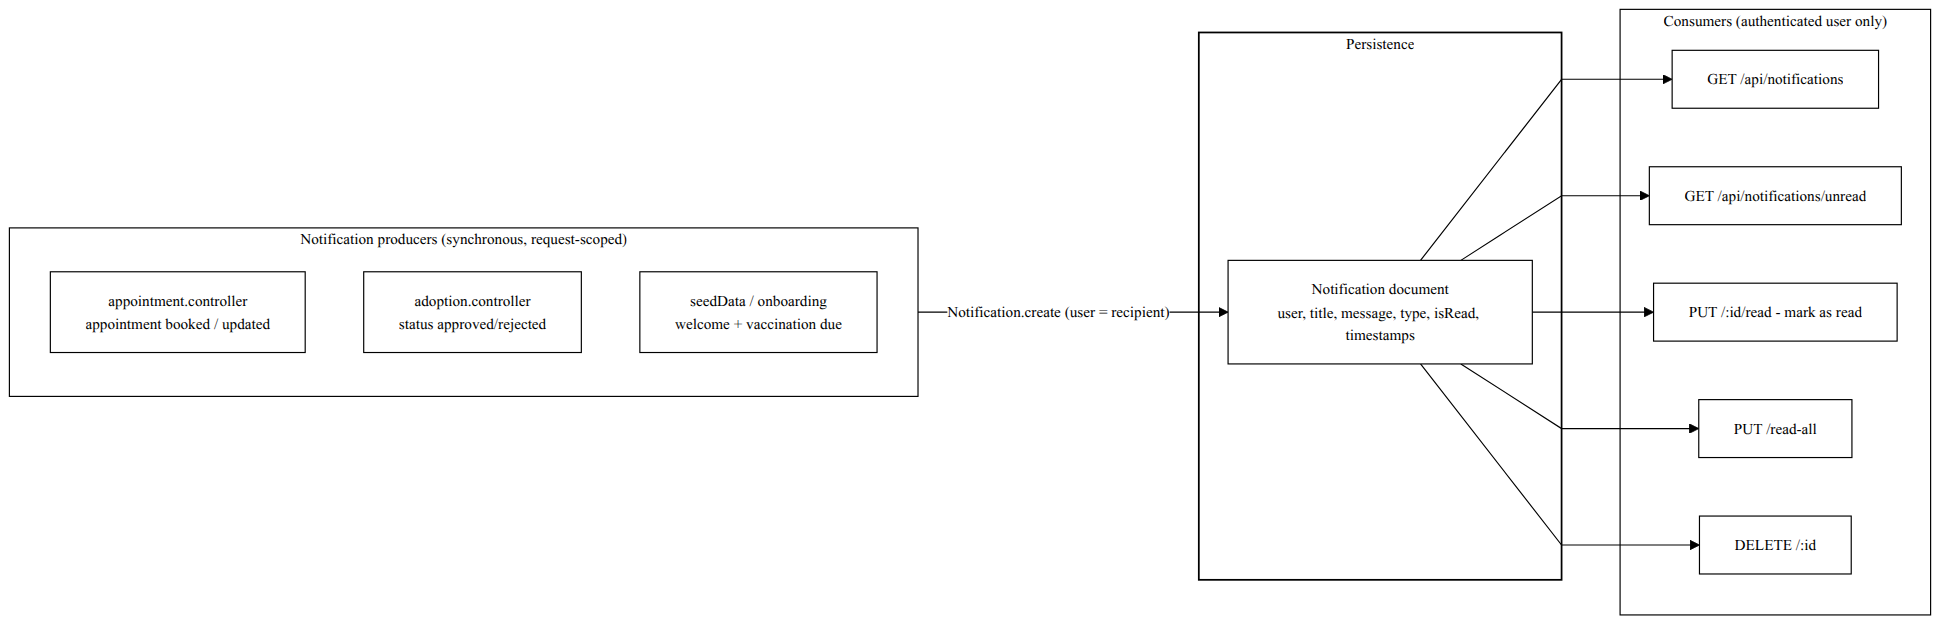
\includegraphics[width=\textwidth]{figures/17-notification-flow.png}
    \caption{Notification creation and consumption flow.}
    \label{fig:notifflow}
\end{figure}

Notifications are the shared feedback channel of the platform. They are created
by the adoption and appointment controllers and read through the notification
API, which is scoped to the owner and supports an unread filter, mark-as-read,
mark-all-as-read, and deletion. The read state persists, so notifications remain
correctly unread/read across reloads.

\begin{figure}[htbp]
    \centering
    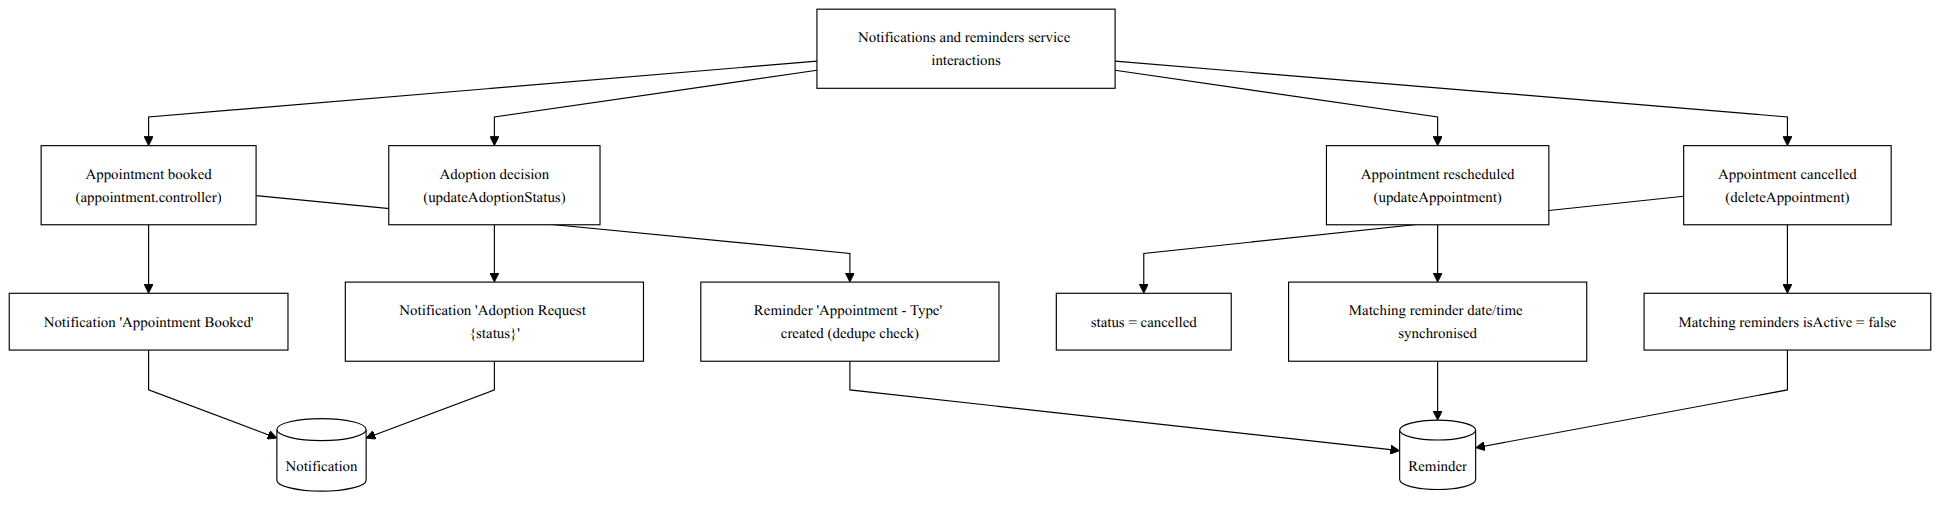
\includegraphics[width=\textwidth]{figures/20-notif-reminder-sync.png}
    \caption{Synchronization between appointments, notifications, and reminders.}
    \label{fig:notifrem}
\end{figure}

The synchronization diagram is a summary of the invariant demonstrated by the
implementation: booking creates the notification and reminder; rescheduling
moves the reminder; cancellation flips the appointment state and deactivates the
reminder. No background job is involved; all effects are applied synchronously
in the request handler against the same MongoDB store.

\section{PetGPT -- the AI Assistant}

\begin{figure}[htbp]
    \centering
    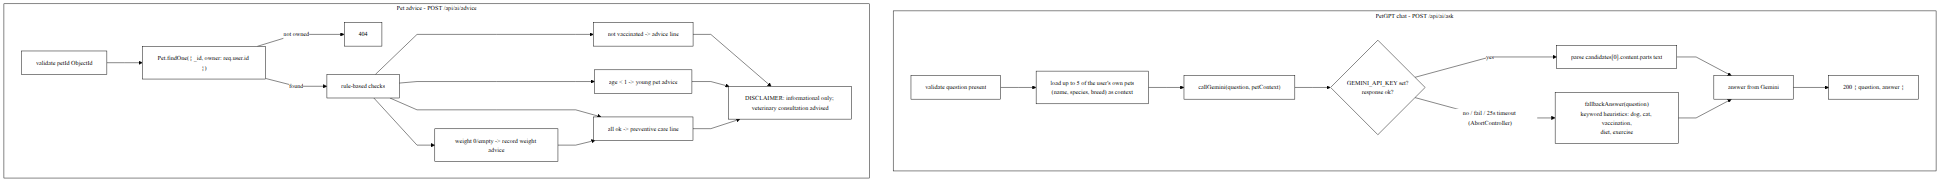
\includegraphics[width=\textwidth]{figures/18-ai-pipeline.png}
    \caption{PetGPT request pipeline with fallback.}
    \label{fig:aipipe}
\end{figure}

The AI subsystem exposes two endpoints. \texttt{POST /api/ai/ask} takes a
question, loads up to five of the user's own pets (name, species, breed) as
context, and calls the Google Gemini REST endpoint
(\texttt{gemini-1.5-flash}) with a PetGPT system instruction and a 25-second
timeout through an \texttt{AbortController}. If the API key is missing, the
call fails, or times out, a built-in keyword fallback returns safe generic
guidance for common topics (dogs, cats, vaccination, diet, exercise). The
second endpoint, \texttt{POST /api/ai/advice}, is fully rule-based: it requires
a pet owned by the user and produces advice from the pet's actual
\texttt{vaccinated} flag, age, and weight, recommending professional veterinary
care when a vaccination or weight record is missing. The assistant therefore
never fabricates a diagnosis; its output is either model-generated general
advice or profile-derived advice from real records.

\section{Community and Lost-and-Found}

\texttt{POST /api/community} creates a post (optionally with an image) bound to
the authenticated user. Likes and comments are embedded arrays; like toggling
adds or removes the user reference, so re-pressing a like cancels it. Posts are
listed publicly, but only when \texttt{isActive: true}. Post, comment, and
lost-and-found report deletion allow either the owner or an administrator.
Lost-and-found reports carry type (\texttt{lost}/\texttt{found}), pet
attributes, location, date, and contact details, with an
\texttt{active}/\texttt{resolved} status that administrators can update.
Ownership checks are identical in shape to the other subsystems: the report is
queried with the owner predicate and the controller verifies
\texttt{report.user} against \texttt{req.user.id} before modification.

\section{Feature Verification Summary}

Each feature described in this chapter was exercised end-to-end in the test
campaign of Chapter~\ref{ch:testing}: pets and QR, favourites, adoption through
to admin approval, appointments with automatic notification and reminder
creation, cancellation deactivating the reminder, community posts with images,
likes and comments, lost-and-found reporting, health records, vaccinations, and
notifications. The persistence, read-back, and cleanup behaviour of every
feature was verified against MongoDB.
\famichapter{Implementation}{This chapter describes how FamiPet is implemented in
code: the repository layout, the backend structure, the data persistence
patterns, and the frontend structure.}{ch:impl}

\section{Repository Layout}

The repository follows a conventional monorepo layout for an Express backend and
a browser frontend:

\begin{center}
\begin{tabular}{@{}p{4.6cm}p{10.0cm}@{}}
\toprule
\textbf{Directory} & \textbf{Content} \\
\midrule
\texttt{backend/} & Express API; subdirectories \texttt{config},
\texttt{controllers}, \texttt{middleware}, \texttt{models}, \texttt{routes},
\texttt{utils}, \texttt{uploads}, and the entry point \texttt{server.js}. \\
\texttt{frontend-react/} & The React~\cite{react} + TypeScript + Vite~\cite{vite} + Tailwind~\cite{tailwind} client,
the project frontend; roadmap phases 1--22 delivered. \\
\texttt{docs/} & \texttt{ROADMAP.md} (phase plan and
status), \texttt{design.md}; this black book lives under
\texttt{docs/blackbook/}. \\
\texttt{AGENTS.md}, \texttt{BASELINE.md}, \texttt{Step10-Report.md},
\texttt{test-email.js} & Project rules, baseline, and verification evidence. \\
\bottomrule
\end{tabular}
\end{center}

\section{Backend Implementation}

The backend runs from a single entry point. \texttt{server.js} applies Helmet,
compression, the CORS origin guard, JSON and URL-encoded body parsing (50\,MB
limit), and development logging; connects to MongoDB; registers a health route,
sixteen route modules under \texttt{/api}, static \texttt{/uploads}; serves
the client build statically on the client port; and ends with a JSON error handler and a
404 handler.

\begin{itemize}
    \item \textbf{Routes} (\path{routes/}) declare the HTTP surface and bind
    middleware (\path{protect}, \path{adminOnly}, \path{upload}) to each
    handler. Public read-only endpoints (pets, breeds, veterinarians,
    community posts, lost-and-found) carry no protection.
    \item \textbf{Controllers} (\path{controllers/}) implement validation,
    ownership checks, business effects, and responses. The authentication
    controller is the largest (roughly 1\,280 lines); the admin controller
    aggregates statistics and moderation operations.
    \item \textbf{Middleware} (\path{middleware/}) provides JWT
    authentication and role checks (\path{auth.js}), the error handler
    (\path{errorHandler.js}) that maps CastErrors to 404, duplicate-key
    errors to 400, and Mongoose validation errors to 400, and the Multer
    upload filter.
    \item \textbf{Models} (\path{models/}) declare the thirteen schemas with
    required fields, enums, default values, the unique indexes, and the bcrypt
    pre-save hook.
    \item \textbf{Config} (\texttt{config/}) centralizes the database
    connection, the Nodemailer transporter, the Gemini client, and Cloudinary.
    \item \textbf{Utilities} (\texttt{utils/}) provide the database seed data
    (breeds, an administrator account, and a demo user).
\end{itemize}

\section{Persistence Pattern}

Every state-changing flow follows the same pattern, which guarantees that what
the UI shows after a reload is what the backend wrote:

\begin{enumerate}
    \item the client sends a request with the bearer token;
    \item the controller validates input and ownership against the database;
    \item documents are created or updated through the Mongoose models;
    \item derived effects (notifications, reminders, pet status transitions)
    are applied as further document writes;
    \item the response returns the persisted data, and the client re-fetches
    the list from the API whenever it must reflect the new state.
\end{enumerate}

This pattern was verified for every feature in the persistence test campaign
(Chapter~\ref{ch:testing}).

\section{Frontend Structure}

The React client implements the user interface in phases driven by the roadmap.
Phases 1--22 (scaffold, Tailwind, assets, routing,
global styles, shared layouts, authentication, dashboard, pet management,
health, vaccinations, appointments, veterinarians, reminders, community,
lost-and-found, favorites, adoption, breeds, settings, admin panel, PetGPT
frontend) are
implemented and committed. Notifications are delivered inside phases 10--14
through shared notification components. Phases 23--29 (API
integration layer, authentication/state consolidation, UI/UX completion,
visual regression, functional regression, Docker/Nginx integration, client
consolidation) are planned and not yet implemented.

The React client consumes the same \texttt{/api} endpoints described in
this black book, so the backend API remains the single source of truth.
\famichapter{Testing and Validation}{This chapter records the testing performed
on FamiPet and the evidence available in the repository. Tests are reported as
they were executed; no unverified result is claimed.}{ch:testing}

\section{Testing Approach}

The project does not ship an in-repository automated test suite. Runtime
verification was performed through dedicated browser and persistence test
scripts against a live backend and database, and the complete evidence was
written to \texttt{Step10-Report.md} (dated 09-09-2026), following the
structured, evidence-oriented reporting convention of~\cite{ieee}. That campaign ran
against the backend at \texttt{localhost:5000} and the frontend at
\texttt{localhost:5502}. The campaign covered four areas: a headless-Chrome
sweep of all screens, an end-to-end persistence verification of every feature,
an administrator test, and a security boundary test.

\section{Browser Sweep}

All 31 interface screens were scanned in a headless Chrome session at the exact
frontend origin: 6 public screens, 13 user screens, and 6 admin screens, plus
repeated views for breed details and pet health. The sweep reported zero
console errors, zero page errors, and zero failed API calls across every page.

\section{Database Persistence Verification}

The table below records the persistence evidence per feature. Each row reflects
an end-to-end check: the API call created the record, the record was found in
the database, the read-back through the API rendered in the UI, and where
applicable deletion or cleanup was verified.

\begin{center}
\begin{longtable}{@{}p{3.4cm}p{3.6cm}p{7.6cm}@{}}
\caption{Database persistence evidence.}
\label{tab:persistence}\\
\toprule
\textbf{Feature} & \textbf{Result} & \textbf{Verified evidence} \\
\midrule
Register + e-mail verify & PASS & 201; SHA-256 token and expiry stored; login
works after verification. \\
Login / profile update & PASS & Name and city persisted; \texttt{/auth/me}
reflects them. \\
Change / reset password & PASS & New bcrypt \texttt{\$2a\$12\$} hash stored;
login with the new password succeeds. \\
Profile picture & PASS & Avatar URL persisted on the user document and the image
renders in the browser. \\
Pets CRUD + QR & PASS & Document and \texttt{qrCode} persisted; shown in
\texttt{/pets/my} as a PNG data URL; delete works. \\
Favourites & PASS & Persisted in the user favourites collection; toggling off
returns the count to zero. \\
Adoption request & PASS & Created in \texttt{Pending} state; listed in
\texttt{/adoptions/my}; admin approval works. \\
Appointment & PASS & Document persisted; booking automatically created a
notification and a reminder; cancellation deactivated the reminder. \\
Reminders & PASS & Created, listed, and completion persisted. \\
Community post (image) & PASS & Post and image URL persisted; like increments,
comment added, public read works; delete works. \\
Lost and found (image) & PASS & Created \texttt{active}; document and image
persisted; listing and status resolution work. \\
Health records & PASS & Created, read, updated, deleted. \\
Vaccinations & PASS & Created, read, upcoming list, updated, deleted. \\
Notifications & PASS & Appointment auto-notification persisted; read /
read-all persisted. \\
Breeds & PASS & 12 breeds with full data displayed as cards and details. \\
\bottomrule
\end{longtable}
\end{center}

\section{Administrator Tests}

The administrator campaign executed against the admin panel and confirmed:
dashboard statistics (9 users, 12 pets, 11 available, 1 adopted, pending
adoptions, lost-and-found summaries), the users list and recent users, pets
management with owner information, adoption approval (status becomes
\texttt{Approved}, the pet is automatically marked adopted, and a notification
is sent to the applicant), lost-and-found status resolution and restore, and
community post deactivation and deletion. All passed.

\section{Security Tests}

\begin{center}
\begin{longtable}{@{}p{3.6cm}p{3.4cm}p{7.6cm}@{}}
\caption{Security test evidence.}
\label{tab:security-tests}\\
\toprule
\textbf{Scenario} & \textbf{Result} & \textbf{Observed behaviour} \\
\midrule
Regular user calls admin routes & PASS & Nine administrative/privileged
endpoints each returned 403 for a regular account. \\
Ownership isolation & PASS & A user could not read, update (404), or cancel
(404) another user's appointment; APIs are owner-scoped. \\
Password hashing & PASS & bcrypt \texttt{\$2a\$12\$} hashes verified directly in
the database for both user and admin accounts. \\
Invalid token & PASS & Garbage JWT returns 401; missing token returns 401 on
protected routes. \\
CORS & PASS & Only the accept-origin guard permits requests; preflight OPTIONS
returns 204 with Authorization and Content-Type allowed. \\
Secret handling & PASS & No API keys in frontend files; keys live only in the
git-ignored \texttt{backend/.env}; only placeholder \texttt{.env.example} is
committed; no secrets in repository history. \\
\bottomrule
\end{longtable}
\end{center}

\section{Defects Found and Fixed}

The campaign surfaced one real defect: uploaded images were blocked by the
browser (\texttt{ERR\_BLOCKED\_BY\_RESPONSE.NotSameOrigin}). The cause was
Helmet's default \texttt{Cross-Origin-Resource-Policy: same-origin}, which
prevented the frontend origin from embedding images served by the backend.
The fix set \path{crossOriginResourcePolicy: \{ policy: "cross-origin" \}} in
\path{backend/server.js}. After the fix, avatar and
community images rendered (\texttt{naturalWidth > 0}) and the full screen sweep
was re-run with zero issues. This is the only backend change recorded; the fix
is part of the current implementation described in Chapter~\ref{ch:arch}.

\section{Test Artifacts}

The automated scripts used for the campaign (\texttt{step10-auth.js},
\texttt{step10-data.js}, \texttt{step10-admin.js}, \texttt{step10-pages.js})
reported zero failures across the auth flow, database persistence, admin and
security suites, and the 31-page browser sweep. The script files lived in a
temporary working directory used for the evaluation and are not part of the
repository; the results are recorded in \texttt{Step10-Report.md} in the
repository root.
\famichapter{Development Process}{This chapter documents how FamiPet was
developed: the workflow rules, the phase-based roadmap, and the project
timeline reconstructed from the repository history.}{ch:process}

\section{Development Workflow}

The project follows the workflow encoded in \texttt{AGENTS.md}: inspect before
changing, treat the backend as the source of truth for identity and ownership,
preserve existing functionality, use real data only, persist through the
database, enforce security on the backend, make the smallest correct change,
test the complete flow, and never claim unverified results. Each phase of work
is completed as an atomic unit: inspect, implement, test, fix failures, update
documentation, commit, tag and push when specified, verify a clean working
tree, and stop.

Every change must reuse existing models, routes, controllers, and utilities
instead of duplicating endpoints or bypassing authentication. The role and
ownership of every resource are enforced on the backend, never by hiding UI
controls. The disciplined, phase-based engineering practices follow the
software-engineering fundamentals collected by~\cite{sommerville}.

\section{Phase-Based Roadmap}

The implementation is tracked in \texttt{ROADMAP.md} as numbered phases. The
frontend phase status below is taken directly from the roadmap. Each
implemented phase is delivered as an atomic commit; the \emph{Commit} column
records the feature commit that completes the phase.

\begin{center}
\begin{longtable}{@{}p{1.2cm}p{5.4cm}p{1.6cm}p{3.4cm}@{}}
\caption{Roadmap phase status.}
\label{tab:phases}\\
\toprule
\textbf{Phase} & \textbf{Name} & \textbf{Status} & \textbf{Commit} \\
\midrule
1 & Scaffold (Vite + React + TS) & Complete & \texttt{80cc21d} \\
2 & Tailwind setup & Complete & \texttt{80cc21d} \\
3 & Assets and theme & Complete & \texttt{80cc21d} \\
4 & Routing & Complete & \texttt{c5f23f3} \\
5 & Global styles and shared layout & Complete & \texttt{be87712} \\
6 & Shared layout components & Complete & \texttt{1a2cf5e} \\
7 & Authentication & Complete & \texttt{9b44727} \\
8 & Dashboard & Complete & \texttt{d2f6952} \\
9 & Pet management & Complete & \texttt{38c6aa9} \\
10 & Health & Complete & \texttt{17fc630} \\
11 & Vaccinations & Complete & \texttt{3d10701} \\
12 & Appointments & Complete & \texttt{e003c98} \\
13 & Veterinarians & Complete & \texttt{721f03f} \\
14 & Reminders & Complete & \texttt{56a1c29} \\
15 & Community & Complete & \texttt{5dd0fef} \\
16 & Lost \& found & Complete & \texttt{d637cd9} \\
17 & Favourites & Complete & \texttt{d7a6f10} \\
18 & Adoption & Complete & \texttt{70293d0} \\
19 & Pet breeds & Complete & \texttt{526f78e} \\
20 & Settings & Complete & \texttt{ed4d6cb} \\
21 & Admin panel & Complete & \texttt{d18c336} \\
22 & AI / PetGPT frontend & Complete & \texttt{d26e955} \\
23 & API integration layer & Planned & --- \\
24 & Auth / state consolidation & Planned & --- \\
25 & UI/UX completion & Planned & --- \\
26 & Visual regression & Planned & --- \\
27 & Functional regression & Planned & --- \\
28 & Docker / Nginx integration & Planned & --- \\
29 & Client consolidation & Planned & --- \\
\bottomrule
\end{longtable}
\end{center}

\section{Timeline and Project Gantt}

The project was initiated in July 2026. The initial period (July and August)
covered planning, requirements analysis, and design, and is recorded in the
project documentation; the repository itself does not carry those commits. The
version-controlled implementation begins on 2026-09-07 with the backend
commits. The Step-10 verification campaign was executed on 2026-09-09, and the
React frontend phases were implemented from 2026-09-21 through 2026-09-22,
with phases 23--29 still planned. The roadmap does not record dates, so the
timeline below is reconstructed from the repository history and the documented
project start, following the scheduling conventions of the
PMBOK~\cite{pmbok}; the Gantt chart itself was rendered with
Mermaid~\cite{mermaid}.

\begin{figure}[htbp]
    \centering
    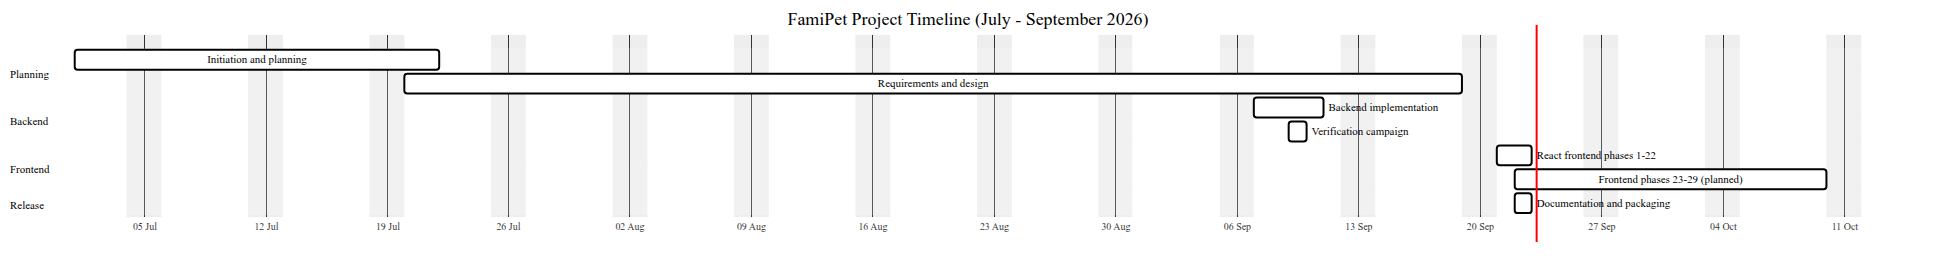
\includegraphics[width=\textwidth]{figures/19-project-gantt.png}
    \caption{Project timeline and Gantt chart (July--September 2026).}
    \label{fig:gantt}
\end{figure}

The key milestones are summarised in Table~\ref{tab:milestones}.

\begin{center}
\begin{longtable}{@{}p{4.2cm}p{3.2cm}p{7.2cm}@{}}
\caption{Key project milestones.}
\label{tab:milestones}\\
\toprule
\textbf{Activity} & \textbf{Period} & \textbf{Evidence} \\
\midrule
Initiation and planning & Jul 2026 & Project brief and design direction. \\
Requirements and design & Jul--Aug 2026 & Requirements, architecture, and
design documentation. \\
Backend implementation & 07--10 Sep 2026 & Initial commits; the sixteen route
modules covering all documented features. \\
Verification campaign & 09 Sep 2026 & \texttt{Step10-Report.md}: browser sweep,
persistence, admin, and security tests. \\
React frontend phases 1--22 & 21--22 Sep 2026 & Roadmap phase table
(Table~\ref{tab:phases}) with commit hashes. \\
Documentation and packaging & 22 Sep 2026 & Black book, project skills, and
graphify artifacts committed. \\
\bottomrule
\end{longtable}
\end{center}
\famichapter{Conclusion and Future Scope}{This chapter summarises what was
delivered, what the verification showed, and the planned future work.}{ch:conclusion}

\section{Summary of the Delivered System}

FamiPet delivers a complete, authenticated pet-care and adoption platform. The
backend, built with Node.js, Express, MongoDB, and Mongoose, exposes sixteen
route modules that cover account management with e-mail verification and secure
password recovery; pet management with a unique digital pet identity and QR
code; health records and vaccinations; veterinary appointment booking with
double-booking protection and automatic notification and reminder creation;
care reminders; favourites; community posts with likes and comments; lost-and-found
reports; adoption applications with administrator approval; a per-user
notification hub; and an AI pet-care assistant grounded in the user's real pet
records.

The system enforces the rules of the project brief on the backend: user identity
comes from the signed token, every user-scoped query binds to the authenticated
user, administrative actions are gated by role, data is persisted in MongoDB
and read back through the API, and validation errors are returned as explicit
HTTP responses. The Step 10 verification campaign confirmed persistence,
ownership isolation, role-based 403s, bcrypt password hashing, JWT handling,
CORS behaviour, and a clean browser sweep over all 31 screens.

\section{Observations}

Three implementation choices deserve emphasis because they affect future work.
First, the AI assistant is the only feature that depends on an external paid
service; it falls back to deterministic guidance when the service is
unavailable, so the platform never breaks. Second, notifications and reminders
are produced synchronously by the controllers, which keeps the system simple and
fully consistent at request time, at the cost of no background scheduling or
real-time push. Third, the React client consumes the backend API as the single
source of truth, so the pages always present exactly the persisted state the
backend returns.

\section{Future Scope}

The planned future work is recorded in the roadmap. The items below are planned,
not implemented.

\begin{center}
\begin{longtable}{@{}p{5.2cm}p{9.4cm}@{}}
\caption{Planned future work.}
\label{tab:planned}\\
\toprule
\textbf{Area} & \textbf{Planned work} \\
\midrule
API integration layer & Phase 23: formal typed API client for the React app. \\
Auth and state management & Phase 24: consolidation of authentication and state
management across migrated pages. \\
UI/UX completion & Phase 25: finish the remaining interface surfaces. \\
Visual regression & Phase 26: pixel-level regression for the frontend UI. \\
Functional regression & Phase 27: end-to-end regression across all features. \\
Docker / Nginx & Phase 28: containerization and reverse-proxy deployment. \\
Client consolidation & Phase 29: decommission the legacy browser client once
regression phases are green. \\
Background scheduling & Considered: convert reminders into scheduled jobs and add
push notifications using the unused \texttt{node-cron} and \texttt{socket.io}
dependencies. \\
Provider expansion & Considered: implement the OpenAI adapter described in
\texttt{.env.example} as an alternative AI provider behind the Google default. \\
\bottomrule
\end{longtable}
\end{center}

\section{Closing Statement}

The black book documents the FamiPet project as it exists in the repository:
its requirements, architecture, data model, security, features, implementation,
testing evidence, and development process. Implemented, planned, and considered
items have been clearly distinguished throughout. The system is feature-complete
on the backend, and the React frontend implements the delivered roadmap phases;
the backend remains the source of truth for all
data and authorization.

% ---------------- REFERENCES ----------------
\famichapterstar{References}{The sources cited in this black book. All references
relate to verified technologies, documentation and literature used in the project.}{ch:refs}
\famibid{references}

% ---------------- APPENDICES ----------------
\famichapterstar{Appendix A -- REST API Summary}{A catalogue of the HTTP surface
exposed by the FamiPet backend, as implemented in the route modules.}{app:a}

\section*{Authentication and Users}

\begin{center}
\begin{longtable}{@{}p{6.2cm}p{2.6cm}p{5.8cm}@{}}
\toprule
\textbf{Endpoint} & \textbf{Method} & \textbf{Access} \\
\midrule
\path{/api/auth/register} & POST & Public \\
\path{/api/auth/login} & POST & Public \\
\path{/api/auth/verify-email/:token} & GET & Public \\
\path{/api/auth/resend-verification} & POST & Public \\
\path{/api/auth/forgot-password} & POST & Public \\
\path{/api/auth/reset-password/:token} & POST & Public \\
\path{/api/auth/me} & GET & Protect \\
\path{/api/auth/profile} & PUT & Protect \\
\path{/api/auth/change-password} & PUT & Protect \\
\path{/api/users} & GET & Protect \\
\path{/api/users/:id} & GET & Public (profile) \\
\path{/api/users/favorites/:petId} & POST & Protect \\
\path{/api/users/avatar} & POST & Protect (upload) \\
\bottomrule
\end{longtable}
\addtocounter{table}{-1}
\end{center}

\section*{Pets, Breeds, and Favourites}

\begin{center}
\begin{longtable}{@{}p{6.2cm}p{2.6cm}p{5.8cm}@{}}
\toprule
\textbf{Endpoint} & \textbf{Method} & \textbf{Access} \\
\midrule
\path{/api/pets} & GET & Public \\
\path{/api/pets/featured} & GET & Public \\
\path{/api/pets/my} & GET & Protect \\
\path{/api/pets} & POST & Protect \\
\path{/api/pets/:id} & GET & Public \\
\path{/api/pets/:id} & PUT / DELETE & Protect (owner) \\
\path{/api/pets/:id/qr} & GET & Protect (owner) \\
\path{/api/breeds} & GET & Public \\
\path{/api/breeds/:id} & GET & Public \\
\path{/api/breeds} & POST & Protect + adminOnly \\
\path{/api/breeds/:id} & PUT / DELETE & Protect + adminOnly \\
\path{/api/favorites} & GET / POST & Protect \\
\path{/api/favorites/:id} & DELETE & Protect \\
\bottomrule
\end{longtable}
\addtocounter{table}{-1}
\end{center}

\section*{Care: Health, Vaccinations, Veterinarians, Appointments, Reminders}

\begin{center}
\begin{longtable}{@{}p{6.2cm}p{2.6cm}p{5.8cm}@{}}
\toprule
\textbf{Endpoint} & \textbf{Method} & \textbf{Access} \\
\midrule
\path{/api/health} & GET / POST & Protect (owner) \\
\path{/api/health/:id} & GET / PUT / DELETE & Protect (owner) \\
\path{/api/vaccinations} & GET / POST & Protect (owner) \\
\path{/api/vaccinations/upcoming} & GET & Protect (owner) \\
\path{/api/vaccinations/:id} & PUT / DELETE & Protect (owner) \\
\path{/api/veterinarians} & GET & Public \\
\path{/api/veterinarians/:id} & GET & Public \\
\path{/api/veterinarians} & POST & Protect + adminOnly \\
\path{/api/veterinarians/:id} & PUT / DELETE & Protect + adminOnly \\
\path{/api/appointments} & GET / POST & Protect (owner) \\
\path{/api/appointments/:id} & PUT / DELETE & Protect (owner) \\
\path{/api/reminders} & GET / POST & Protect (owner) \\
\path{/api/reminders/:id} & PUT / DELETE & Protect (owner) \\
\path{/api/reminders/:id/complete} & PUT & Protect (owner) \\
\bottomrule
\end{longtable}
\addtocounter{table}{-1}
\end{center}

\section*{Community, Lost-and-Found, Adoption, Notifications, AI}

\begin{center}
\begin{longtable}{@{}p{6.2cm}p{2.6cm}p{5.8cm}@{}}
\toprule
\textbf{Endpoint} & \textbf{Method} & \textbf{Access} \\
\midrule
\path{/api/community} & GET & Public (active posts) \\
\path{/api/community/:id} & GET & Public \\
\path{/api/community} & POST & Protect (upload) \\
\path{/api/community/:id} & PUT / DELETE & Protect (owner) \\
\path{/api/community/:id/like} & POST & Protect \\
\path{/api/community/:id/comments} & POST & Protect \\
\path{/api/community/:id/comments/:commentId} & DELETE & Protect (owner) \\
\path{/api/lost-found} & GET & Public \\
\path{/api/lost-found/:id} & GET & Public \\
\path{/api/lost-found} & POST & Protect (upload) \\
\path{/api/lost-found/:id} & PUT / DELETE & Protect (owner or admin) \\
\path{/api/adoptions} & GET & Protect + adminOnly \\
\path{/api/adoptions/my} & GET & Protect (owner) \\
\path{/api/adoptions} & POST & Protect \\
\path{/api/adoptions/:id} & PUT / DELETE & Protect + adminOnly \\
\path{/api/notifications} & GET & Protect (owner) \\
\path{/api/notifications/unread} & GET & Protect (owner) \\
\path{/api/notifications/read-all} & PUT & Protect (owner) \\
\path{/api/notifications/:id/read} & PUT & Protect (owner) \\
\path{/api/notifications/:id} & DELETE & Protect (owner) \\
\path{/api/ai/ask} & POST & Protect \\
\path{/api/ai/advice} & POST & Protect \\
\bottomrule
\end{longtable}
\addtocounter{table}{-1}
\end{center}

\section*{Admin}

\begin{center}
\begin{longtable}{@{}p{6.2cm}p{2.6cm}p{5.8cm}@{}}
\toprule
\textbf{Endpoint} & \textbf{Method} & \textbf{Access} \\
\midrule
\path{/api/admin/dashboard} & GET & Protect + adminOnly \\
\path{/api/admin/users} & GET & Protect + adminOnly \\
\path{/api/admin/users/recent} & GET & Protect + adminOnly \\
\path{/api/admin/users/:id/block} & PUT & Protect + adminOnly \\
\path{/api/admin/users/:id} & DELETE & Protect + adminOnly \\
\path{/api/admin/pets} & GET & Protect + adminOnly \\
\path{/api/admin/pets/:id} & DELETE & Protect + adminOnly \\
\path{/api/admin/lost-found} & GET & Protect + adminOnly \\
\path{/api/admin/lost-found/:id/status} & PUT & Protect + adminOnly \\
\path{/api/admin/lost-found/:id} & DELETE & Protect + adminOnly \\
\path{/api/admin/community} & GET & Protect + adminOnly \\
\path{/api/admin/community/:id/status} & PUT & Protect + adminOnly \\
\path{/api/admin/community/:id} & DELETE & Protect + adminOnly \\
\bottomrule
\end{longtable}
\addtocounter{table}{-1}
\end{center}

\section*{System}

\begin{center}
\begin{longtable}{@{}p{6.2cm}p{2.6cm}p{5.8cm}@{}}
\toprule
\textbf{Endpoint} & \textbf{Method} & \textbf{Access} \\
\midrule
\path{/api/status} & GET & Public (health check) \\
\path{/} & GET & Public (service banner) \\
\path{/uploads/*} & GET & Public (static images) \\
\bottomrule
\end{longtable}
\addtocounter{table}{-1}
\end{center}
\famichapterstar{Appendix B -- Configuration}{The runtime configuration of the
FamiPet backend, as declared in \texttt{backend/.env.example} and read by the
code.}{app:b}

\section*{Environment Variables}

\begin{center}
\begin{longtable}{@{}p{3.6cm}p{3.0cm}p{8.0cm}@{}}
\toprule
\textbf{Variable} & \textbf{Default} & \textbf{Purpose} \\
\midrule
\path{PORT} & \texttt{5000} & HTTP port for the API process. \\
\path{MONGODB\_URI} & \path{mongodb://localhost:27017/animal\_planet} &
MongoDB connection string. \\
\path{JWT\_SECRET} & (required) & Secret used to sign and verify bearer
tokens. \\
\path{JWT\_EXPIRE} & \texttt{30d} & Token expiry duration. \\
\path{CLIENT\_URL} & \path{http://localhost:5500} & Frontend origin(s),
comma-separated, used by CORS and e-mail links. \\
\path{GEMINI\_API\_KEY} & (optional) & Google Gemini key; the PetGPT pipeline
falls back to built-in answers when absent. \\
\path{EMAIL\_SERVICE} & \texttt{gmail} & Nodemailer service name. \\
\path{EMAIL\_USER} & (SMTP) & Sender account for Nodemailer. \\
\path{EMAIL\_PASS} & (SMTP) & App password for the e-mail account.
\\
\path{CLOUDINARY\_CLOUD\_NAME} & (optional) & Cloudinary account for image
hosting. \\
\path{CLOUDINARY\_API\_KEY} & (optional) & Cloudinary API key. \\
\path{CLOUDINARY\_API\_SECRET} & (optional) & Cloudinary API secret. \\
\path{PETGPT\_PROVIDER} & (commented) & Declared OpenAI option; the active
implementation uses the Google provider only. \\
\bottomrule
\end{longtable}
\addtocounter{table}{-1}
\end{center}

\section*{Startup and Defaults}

The backend binds the API to \texttt{PORT} (default 5000). It connects to
MongoDB through \texttt{MONGODB\_URI}; if the variable is missing the connection
falls back to the local default in \texttt{server.js}. The server also listens
on the client port to serve the frontend directory as a fallback when the Live
Server/Vite dev server is not running; if that port is already in use the
fallback is skipped silently. The \texttt{uploads} directory is served
statically at \texttt{/uploads}, and \texttt{CLIENT\_URL} (or an allowed origin)
is used to build the verify-e-mail and reset-password links sent by e-mail.

\section*{Seed Data}

The \texttt{seedData.js} utility populates the database with the breed
catalogue, an administrator account, a demo user account, two veterinarians with
clinics and availability, and a set of sample appointments, adoption requests,
and notifications so the application can be evaluated immediately after setup.

\end{document}